\documentclass[10pt,landscape]{article}
\usepackage{multicol}
\usepackage{calc}
\usepackage{ifthen}
\usepackage[landscape]{geometry}
\usepackage{hyperref}

\usepackage[OT1]{fontenc}
\usepackage[sc]{mathpazo}
\usepackage[utf8]{inputenc}
\usepackage[german]{babel}
\usepackage{amsmath}
\usepackage{amsfonts}
\usepackage{amssymb}
\usepackage{mathtools}
\usepackage{fancyhdr}
\usepackage{setspace}
\usepackage{listings}
\usepackage{stmaryrd}
\usepackage{graphicx}
\usepackage{changepage}
\usepackage{enumitem}
\usepackage{wrapfig}
\usepackage{tikz} 
\usepackage{xcolor, soul}
\newcommand{\green}[1]{\sethlcolor{green}\hl{#1}}
\newcommand{\yellow}[1]{\sethlcolor{yellow} \hl{#1}}
\newcommand{\blue}[1]{\sethlcolor{cyan} \hl{#1}}


% To make this come out properly in landscape mode, do one of the following
% 1.
%  pdflatex latexsheet.tex
%
% 2.
%  latex latexsheet.tex
%  dvips -P pdf  -t landscape latexsheet.dvi
%  ps2pdf latexsheet.ps


% If you're reading this, be prepared for confusion.  Making this was
% a learning experience for me, and it shows.  Much of the placement
% was hacked in; if you make it better, let me know...


% 2008-04
% Changed page margin code to use the geometry package. Also added code for
% conditional page margins, depending on paper size. Thanks to Uwe Ziegenhagen
% for the suggestions.

% 2006-08
% Made changes based on suggestions from Gene Cooperman. <gene at ccs.neu.edu>


% To Do:
% \listoffigures \listoftables
% \setcounter{secnumdepth}{0}


% This sets page margins to .5 inch if using letter paper, and to 1cm
% if using A4 paper. (This probably isn't strictly necessary.)
% If using another size paper, use default 1cm margins.
\ifthenelse{\lengthtest { \paperwidth = 11in}}
	{ \geometry{top=.5in,left=.5in,right=.5in,bottom=.5in} }
	{\ifthenelse{ \lengthtest{ \paperwidth = 297mm}}
		{\geometry{top=1cm,left=1cm,right=1cm,bottom=1cm} }
		{\geometry{top=1cm,left=1cm,right=1cm,bottom=1cm} }
	}

% Turn off header and footer
\setcounter{page}{1}


% Redefine section commands to use less space
\makeatletter
\renewcommand{\section}{\@startsection{section}{1}{0mm}%
                                {-1ex plus -.5ex minus -.2ex}%
                                {0.5ex plus .2ex}%x
                                {\normalfont\large\bfseries}}
\renewcommand{\subsection}{\@startsection{subsection}{2}{0mm}%
                                {-1explus -.5ex minus -.2ex}%
                                {0.5ex plus .2ex}%
                                {\normalfont\normalsize\bfseries}}
\renewcommand{\subsubsection}{\@startsection{subsubsection}{3}{0mm}%
                                {-1ex plus -.5ex minus -.2ex}%
                                {1ex plus .2ex}%
                                {\normalfont\small\bfseries}}
\makeatother

% Define BibTeX command
\def\BibTeX{{\rm B\kern-.05em{\sc i\kern-.025em b}\kern-.08em
    T\kern-.1667em\lower.7ex\hbox{E}\kern-.125emX}}

% Don't print section numbers
\setcounter{secnumdepth}{0}


\setlength{\parindent}{0pt}
\setlength{\parskip}{0pt plus 0.5ex}


% -----------------------------------------------------------------------

\begin{document}
\raggedright
\footnotesize
\begin{multicols}{3}


% multicol parameters
% These lengths are set only within the two main columns
%\setlength{\columnseprule}{0.25pt}
\setlength{\premulticols}{1pt}
\setlength{\postmulticols}{1pt}
\setlength{\multicolsep}{1pt}
\setlength{\columnsep}{2pt}

\begin{center}
     \Large{\textbf{Analysis 1 - Cheat Sheet}} \\
\end{center}

\section{Reelle Zahlen, Euklidische Räume, Komplexe Zahlen}
\subsection{Der Körper der reellen Zahlen}
\yellow{Satz 1.1:} Es gibt keine Gleichung der Form
$x^{n}+a_{n-1} x^{n-1}+\cdots+a_{0}=0$ mit $a_{i} \in \mathbb{Q}$, so dass $x=\pi$ eine Lösung ist. \\
\yellow{Satz 1.2:} $\mathbb{R}$ ist ein kommutativer, angeordneter Körper, der ordnungsvollständig ist.\\
\textbf{Axiome der Addition:}\\
A1: Assoziativität  $x+(y+z)=(x+y)+z \forall x, y, z \in \mathbb{R}$ \\
A2: Neutrales Element  $x+0=x \quad \forall x \in \mathbb{R}$ \\
A3: Inverses Element $\forall x \in \mathbb{R} \exists y \in \mathbb{R}: \quad x+y=0$\\
A4: Kommutativität  $x+z=z+x \quad \forall x, z \in \mathbb{R}$\\
\textbf{Axiome der Multiplikation:}\\
M1: Assoziativität $\quad x \cdot(y \cdot z)=(x \cdot y) \cdot z \quad \forall x, y, z \in$ \\
M2: Neutrales Element $\quad x \cdot 1=x \quad \forall x \in \mathbb{R}$ \\
M3: Inverses Element $\quad \forall x \in \mathbb{R}, \quad x \neq 0 \quad \exists y \in \mathbb{R}: \quad x \cdot y=1$\\
M4: Kommutativität $\quad x \cdot z=z \cdot x \quad \forall x, z \in \mathbb{R}$\\
\textbf{Distributivität:}\\
D1: $\quad x \cdot(y+z)=x \cdot y+x \cdot z \quad \forall x, y, z \in \mathbb{R}$\\
\textbf{Ordnungsaxiome:}\\
O1: Reflexivität $\quad x \leq x \quad \forall x \in \mathbb{R}$\\
O2: Transitivität $\quad x \leq y$ und $y \leq z \Longrightarrow x \leq z$\\
O3: Antisymmetrie $x \leq y$ und $y \leq x \Longrightarrow x=y$\\
O4: Total  $\forall x, y \in \mathbb{R} \text { gilt entweder } x \leq y \text { oder } y \leq x$\\
\textbf{Kompatibilität:}\\
K1: $\forall x, y, z \in \mathbb{R}: \quad x \leq y \Longrightarrow x+z \leq y+2$\\
K2: $\forall x \geq 0, \quad \forall y \geq 0: \quad x \cdot y \geq 0$\\
\textbf{Ordnungsvollständigkeit:}\\
Seien $A, B$ Teilmengen von $\mathbb{R}$, so dass
\begin{enumerate}[label=(\roman*)]
    \item $A \neq \emptyset, \quad B \neq \emptyset$
    \item $\forall a \in A$ und $\forall b \in B$ gilt: $a \leq b$
\end{enumerate}
Dann gibt es $c \in \mathbb{R}$, so dass $\forall a \in A: a \leq c$ und $>: \forall b \in B: c \leq b$.\\
\green{Korollar 1.6.:}\\
1. Eindeutigkeit der additiven und multiplikativen Inverse. \\
2. $0 \cdot x=0 \quad \forall x \in \mathbb{R}$ \\
3. $(-1) \cdot x=-x \quad \forall x \in \mathbb{R}$, insbesondere $(-1)^{2}=1$ \\
4. $y \geq 0 \Longleftrightarrow(-y) \leq 0$ \\
5. $y^{2} \geq 0 \quad \forall y \in \mathbb{R}$, insbesondere $1=1 \cdot 1 \geq 0$ \\
6. $x \leq y$ und $u \leq v \Longrightarrow x+u \leq y+v$ \\
7. $0 \leq x \leq y$ und $0 \leq u \leq v \Longrightarrow x \cdot u \leq y \cdot v$ \\
\green{Korollar 1.7 (Archimedisches Prinzip):} Sei $x \in \mathbb{R}$ mit $x>0$ und $y \in \mathbb{R} .$ Dann gibt es $n \in \mathbb{N}$ mit $y \leq n \cdot x$. \\
\yellow{Satz 1.8.:} Für jedes $t \geq 0, t \in \mathbb{R}$ hat die Gleichung $x^{2}=t$ eine Lösung in $\mathbb{R}$.\\
\textbf{Bemerkung:} Für $t \geq 0$ gibt es genau eine Lösung von $x^{2}=t$ mit $x \geq 0$. Sie wird mit $\sqrt{t}$ bezeichnet. \\
\blue{Definition 1.9.:} Seien $x, y \in \mathbb{R}$:
\begin{enumerate}[label=(\roman*)]
    \item $\max \{x, y\}=\left\{\begin{array}{lll}x & \text { falls } & y \leq x \\ y & \text { falls } & x \leq y\end{array}\right.$ 
    \item $\min \{x, y\}=\left\{\begin{array}{lll}y & \text { falls } & y \leq x \\ x & \text { falls } & x \leq y\end{array}\right.$
    \item Der Absolutbetrag einer Zahl $x \in \mathbb{R}:|x|=\max \{x,-x\}$
\end{enumerate}
\yellow{Satz 1.10.:} 
\begin{enumerate}[label=(\roman*)]
    \item $|x| \geq 0 \quad \forall x \in \mathbb{R}$
    \item $|x y|=|x||y| \quad \forall x, y \in \mathbb{R}$
    \item $|x+y| \leq|x|+|y| \quad \forall x, y, \in \mathbb{R}$
    \item $|x+y| \geq|| x|-| y|| \quad \forall x, y \in \mathbb{R}$
\end{enumerate}
\yellow{Satz 1.10.:} $\forall \epsilon>0, \quad \forall x, y \in \mathbb{R}$ gilt: $2|x y| \leq \epsilon x^{2}+\frac{1}{\epsilon} y^{2}$. \\
\blue{Definition 1.12:} Sei $A \subseteq \mathbb{R}$ eine Teilmenge.
\begin{enumerate}[label=(\roman*)]
    \item $c \in \mathbb{R}$ ist eine obere Schranke von A falls $\forall a \in A: a \leq c .$ Die Menge A heisst nach oben beschränkt, falls es eine obere Schranke von A gibt.
    \item $c \in \mathbb{R}$ ist eine untere Schranke von A falls $\forall a \in A: c \leq a .$ Die Menge A heisst nach unten beschränkt, falls es eine untere Schranke von A gibt.
    \item  Ein Element $m \in \mathbb{R}$ heisst ein Maximum von A falls $m \in A$ und $m$ eine obere Schranke von A ist.
    \item Ein Element $m \in \mathbb{R}$ heisst ein Minimum von A falls $m \in A$ und $m$ eine untere Schranke von A ist.
\end{enumerate}
\yellow{Satz 1.15:} Sei $A \subseteq \mathbb{R}, A \neq \emptyset$.
\begin{enumerate}[label=(\roman*)]
    \item  Sei $A$ nach oben beschränkt. Dann gibt es eine kleinste obere Schranke von $A$: $c:=\sup A$ genannt das Supremum von $A$.
    \item Sei $A$ nach unten beschränkt. Dann gibt es eine grösste untere Schranke von $A$: $d:=\inf A$ genannt das Infimum von $A$.
\end{enumerate}
\green{Korollar 1.16.:} Seien $A \subseteq B \subseteq \mathbb{R}$ Teilmengen von $\mathbb{R}$.
\begin{enumerate}
    \item Falls $B$ nach oben beschränkt ist, folgt $\sup A \leq \sup B .$
    \item Falls $B$ nach unten beschränkt ist, folgt $\inf B \leq \inf A$.
\end{enumerate}
\subsection{Kardinalität}
\blue{Definition 1.18.:}
\begin{enumerate}[label=(\roman*)]
    \item Zwei Mengen $X, Y$ heissen gleichmächtig, falls es eine Bijektion $f: X \longrightarrow Y$ gibt.
    \item Eine Menge $X$ ist endlich, falls entweder $X=\emptyset$ oder $\exists n \in \mathbb{N}$, so dass $X$ und $\{1,2,3, \ldots, n\}$ gleichmächtig sind. Im ersten Fall ist die Kardinalität von $X$, card $X=0$ und im zweiten Fall ist $\operatorname{card} X=n$.
    \item Eine Menge $X$ ist abzählbar, falls sie endlich oder gleichmächtig wie $\mathbb{N}$ ist.
\end{enumerate}
\yellow{Satz 1.20 (Cantor):} $\mathbb{R}$ ist nicht abzählbar.\\
\subsection{Der Euklidische Raum}
$\mathbb{R}^{n}=\left\{\left(x_{1}, \ldots, x_{n}\right): x_{j} \in \mathbb{R} \quad \forall j\right\}$\\
$x+y:=\left(x_{1}+y_{1}, \ldots, x_{n}+y_{n}\right), \quad \alpha \cdot x:=\left(\alpha x_{1}, \ldots, \alpha x_{n}\right)$\\
$\begin{aligned}
    \mathbb{R} \times \mathbb{R}^{n} & \longrightarrow \mathbb{R}^{n} & \mathbb{R}^{n} \times \mathbb{R}^{n} & \longrightarrow \mathbb{R}^{n} \\
    (\alpha, x) & \longmapsto \alpha \cdot x &(x, y) & \longmapsto x+y
\end{aligned}$\\
\textbf{Skalarprodukt:} $\langle x, y\rangle:=\sum_{j=1}^{n} x_{j} y_{j}$ mit folgenden Eigenschaften: \\
\begin{enumerate}
    \item $\langle x, y\rangle=\langle y, x\rangle \quad \forall x, y \in \mathbb{R}^{n} \quad$ (symmetrisch).
    \item $\left\langle\alpha_{1} x_{1}+\alpha_{2} x_{2}, y\right\rangle=\alpha_{1}\left\langle x_{1}, y\right\rangle+\alpha_{2}\left\langle x_{2}, y\right\rangle \quad \forall \alpha_{1}, \alpha_{2} \in \mathbb{R}, \quad \forall x_{1}, x_{2}, y \in \mathbb{R}^{n} \quad$ (bilinear).
    \item $\langle x, x\rangle=\sum_{i=1}^{n} x_{j}^{2} \geq 0 \quad$ mit Gleichheit genau dann, wenn $x=0$ (positiv definit).
\end{enumerate}
\textbf{Norm: } $\|x\|=\sqrt{\langle x, x\rangle}$ \\
\yellow{Satz 1.21 (Cauchy-Schwarz):} $|\langle x, y\rangle| \leq\|x\| \cdot\|y\| \quad \forall x, y \in \mathbb{R}^{n}$\\
\yellow{Satz 1.22.:}
\begin{enumerate}
    \item $\|x\| \geq 0$ mit Gleichheit genau dann wenn $x=0$.
    \item $\|\alpha \cdot x\|=|\alpha|\|x\| \quad \forall \alpha \in \mathbb{R}, \quad \forall x \in \mathbb{R}^{n}$
    \item $\|x+y\| \leq\|x\|+\|y\| \quad \forall x, y \in \mathbb{R}^{n}$
\end{enumerate}
\textbf{Kreuzprodukt:}
$\begin{aligned}
    f: \mathbb{R}^{3} \times \mathbb{R}^{3} & \longrightarrow \mathbb{R}^{3} \\
    &(a, b) \quad \longmapsto a \times b=\left(a_{2} b_{3}-a_{3} b_{2}, a_{3} b_{1}-a_{1} b_{3}, a_{1} b_{2}-a_{2} b_{1}\right)
\end{aligned}$
Das Kreuzprodukt hat folgende Eigenschaften: $\forall a, b, c \in \mathbb{R}^{3}:$
\begin{enumerate}
    \item $(\mu+b) \times c=a \times c+b \times c \quad$ (Distributivität)
    \item $a \times b=-b \times a \quad$ (Antisymmetrie)
    \item $a \times(b \times c)+c \times(a \times b)+b \times(c \times a)=0 \quad$ (Jacobi-Identität)
\end{enumerate}
\subsection{Komplexe Zahlen}
\textbf{Multiplikation:} $\left(x_{1}, y_{1}\right) \cdot\left(x_{2}, y_{2}\right)=\left(x_{1} x_{2}-y_{1} y_{2}, x_{1} y_{2}+x_{2} y_{1}\right)$\\
\yellow{Satz 1.23:} $\mathbb{R}^{2}$ versehen mit der Addition der Vektoren $+$ und obig definierter Multiplikation ist ein kommutativer Körper mit Einselement $(1,0)$ und Nullelement $(0,0)$. \\
$i = (0,1) \Longleftrightarrow i^{2}=(0,1)(0,1)=(-1,0)=-(1,0)$\\
Für $z=x+y i$ gilt $\bar{z}=x-y i$. \\
\yellow{Satz 1.24.:}
\begin{enumerate}
    \item $\overline{\left(z_{1}+z_{2}\right)}=\bar{z}_{1}+\bar{z}_{2}, \quad \overline{\left(z_{1} z_{2}\right)}=\bar{z}_{1} \bar{z}_{2} \quad \forall z_{1}, z_{2} \in \mathbb{C}$
    \item $z \bar{z}=x^{2}+y^{2}=\|z\|^{2}$
\end{enumerate}
Für $z \neq 0$ folgt somit $z^{-1}=\frac{\bar{z}}{\|z\|^{2}}$.\\
Sei $r=\|z\|$, dann ist $x=r \cos \phi$ und $y=r \sin \phi \Longrightarrow z=r(\cos \phi+i \sin \phi)$. $r=\|z\|$ ist der \textbf{Absolutbetrag}
und $\phi$ das \textbf{Argument} der Zahl $z$. Es gilt:
\begin{enumerate}
    \item $z_{1} z_{2}=r_{1} r_{2}\left(\cos \left(\phi_{1}+\phi_{2}\right)+\sin \left(\phi_{1}+\phi_{2}\right) \cdot i\right)$
    \item $z^{n}=r^{n}(\cos (n \cdot \phi)+i \sin (n \cdot \phi))$
\end{enumerate}
\green{Korollar 1.25.:} Sei $n \in \mathbb{N}, n \geq 1 .$ Dann hat die Gleichung $z^{n}=1$ genau $n$ Lösungen in $\mathbb{C}: z_{1}, z_{2}, \ldots, z_{n}$, wobei 
$z_{j}=\cos \frac{2 \pi j}{n}+i \cdot \sin \frac{2 \pi j}{n}, \quad 1 \leq j \leq n$ \\
\yellow{Satz 1.26 (Fundamentalsatz der Algebra):} Sei $n \geq 1, n \in \mathbb{N}$ und $P(z)=z^{n}+a_{n-1} z^{n-1}+\cdots+a_{0}, \quad a_{j} \in \mathbb{C}$
Dann gibt es $z_{1}, \ldots, z_{n}$ in $\mathbb{C}, s o$ dass $P(z)=\left(z-z_{1}\right)\left(z-z_{2}\right) \cdots\left(z-z_{n}\right)$.\\
\textbf{Mitternachtsformel: } $a x^2 + b x + c = 0 \Longleftrightarrow x_{1,2} = \frac{-b \pm \sqrt{b^2 - 4 a c}}{2 a}$\\
\textbf{pq-Formel: } $x^2 + p x + q = 0 \Longleftrightarrow x_{1,2} = - \frac{p}{2} \pm \sqrt{\left(\frac{p}{2}\right)^2 - q}$
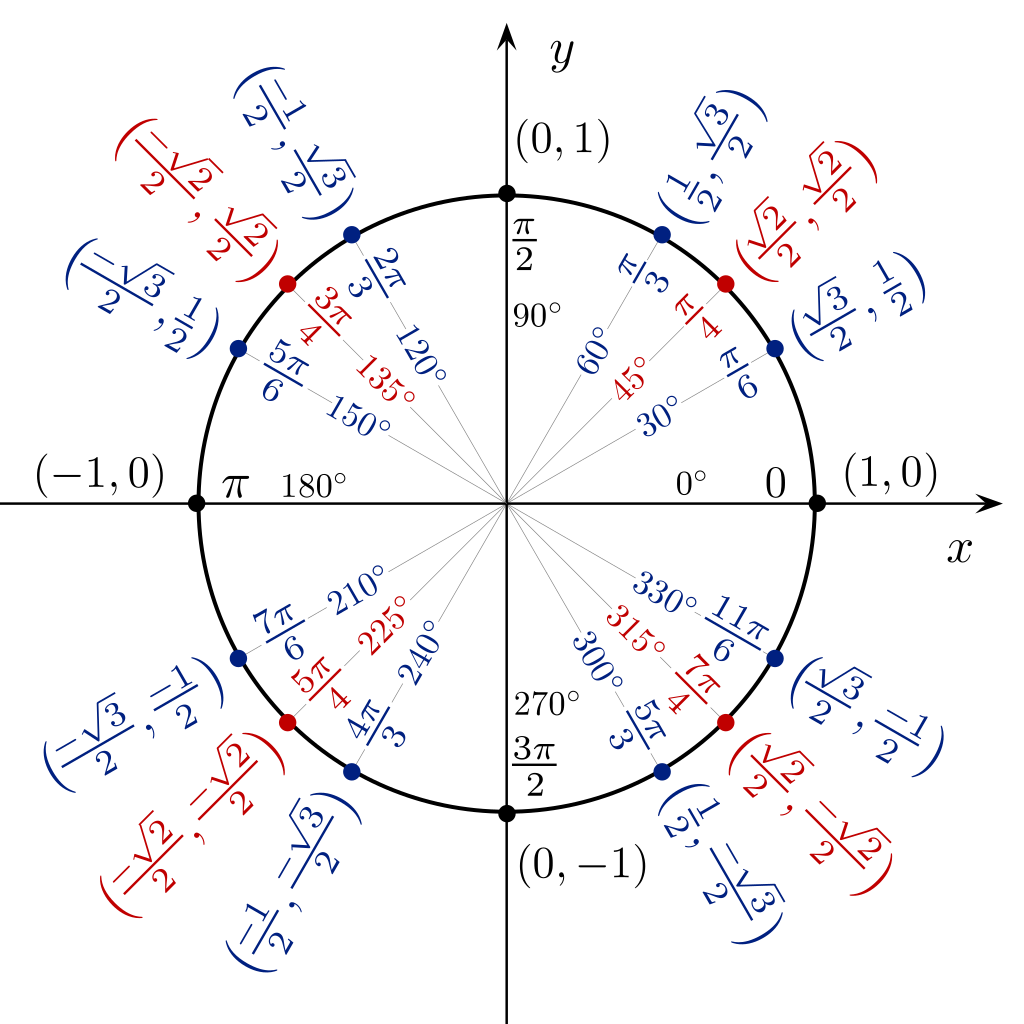
\includegraphics[width = 0.3\textwidth]{unit_circle_angles.png}
\section{Folgen und Reihen}
\subsection{Grenzwert einer Folge}
\blue{Definition 2.1.:} Eine Folge (reller Zahlen) ist eine Abbildung $a: \mathbb{N}^{*} \longrightarrow \mathbb{R} .$
Wir schreiben $a_{n}$ statt a $a(n)$ und bezeichnen eine Folge mit $\left(a_{n}\right)_{n \geq 1}$.\\
\green{Lemma 2.3.:} Sei $\left(a_{n}\right)_{n \geq 1}$ eine Folge. Dann gibt es höchstens eine reelle Zahl $l \in \mathbb{R}$ mit der Eigenschaft:
$\forall \epsilon>0$ ist die Menge $\left\{n \in \mathbb{N}: a_{n} \notin\right] l-\epsilon, l+\mid \epsilon[\}$ endlich. \\
\blue{Definition 2.4.:} Eine Folge $\left(a_{n}\right)_{n \geq 1}$ heisst konvergent, falls es $l \in \mathbb{R}$ gibt, so dass $\forall \epsilon>0$ die Menge
$\left\{n \in \mathbb{N}^{*}: a_{n} \notin\right] l-\epsilon, l+\epsilon[\}$ endlich ist. Somit ist nach Lemma 2.3 eine solche Zahle $l$
eindeutig bestimmt und wir mit $\lim _{n \rightarrow \infty} a_{n}$ bezeichnet und nennt sich Grenzwert 
oder Limes der Folge $\left(a_{n}\right)_{n \geq 1}$. \\
\textbf{Bemerkung 2.5.:} Jede konvergente Folge ist beschränkt: Sei $\left(a_{n}\right)_{n \geq 1}$ konvergent mit Grenzwert $l$. Dann ist $\left\{a_{n}: n \geq 1\right\}$ beschränkt:
Sei $\epsilon=1$ und $\left\{n \in \mathbb{N}^{*}: a_{n} \notin\right] l-1, l+[\}1=\left\{i_{1}, \ldots, i_{M}\right\}$. Dann folgt:
$\left.\left\{a_{n}: n \geq 1\right\} \subseteq\right] l-1, l+1\left[\cup\left\{a_{i_{1}}, \ldots, a_{i_{M}}\right\}\right.$
und ist daher beschränkt. \\
\green{Lemma 2.6.:} Sei $\left(a_{n}\right)_{n \geq 1}$ eine Folge. Folgende Aussagen sind äquivalent:
\begin{enumerate}
        \item $\left(a_{n}\right)_{n \geq 1}$ konvergiert gegen $l=\lim _{n \rightarrow \infty} a_{n}$.
        \item $\forall \epsilon>0 \quad \exists N \geq 1$, so dass $\left|a_{n}-l\right|<\epsilon \quad \forall n \geq N$
\end{enumerate}
\yellow{}{Satz 2.8.:} Seien $\left(a_{n}\right)_{n \geq 1}$ und $\left(b_{n}\right)_{n \geq 1}$ konvergente Folgen mit a $=\lim _{n \rightarrow \infty} a_{n}, b=\lim _{n \rightarrow \infty} b_{n} .$
\begin{enumerate}
        \item Dann ist $\left(a_{n}+b_{n}\right)_{n \geq 1}$ konvergent und $\lim _{n \rightarrow \infty}\left(a_{n}+b_{n}\right)=a+b$.
        \item Dann ist $\left(a_{n} \cdot b_{n}\right)_{n \geq 1}$ konvergent und $\lim _{n \rightarrow \infty}\left(a_{n} \cdot b_{n}\right)=a \cdot b .$
        \item Nehmen wir audem an, dass $b_{n} \neq 0 \quad \forall n \geq 1$ und $b \neq 0$. Dann ist $\left(\frac{a_{n}}{b_{n}}\right)_{n \geq 1}$
        konvergent und $\lim _{n \rightarrow \infty}\left(\frac{a_{n}}{b_{n}}\right)=\frac{a}{b} .$
        \item Folls es ein $K \geq 1$ gibt mit $a_{n} \leq b_{n} \quad \forall n \geq K$ dann folgt $a \leq b .$
\end{enumerate}
\subsection{Der Satz von Weierstrass und Anwendungen}
\blue{Definition 2.10.:} 
\begin{enumerate}
        \item $\left(a_{n}\right)_{n \geq 1}$ ist monoton wachsend falls: $a_{n} \leq a_{n+1} \quad \forall n \geq 1$
        \item $\left(a_{n}\right)_{n \geq 1}$ ist monoton fallend falls: $a_{n+1} \leq a_{n} \quad \forall n \geq 1$
\end{enumerate}
\yellow{Satz $2.11$ (Weierstrass):} 
\begin{itemize}
        \item Sei $\left(a_{n}\right)_{n \geq 1}$ monoton wachsend und nach oben beschränkt. Dann konvergiert $\left(a_{n}\right)_{n \geq 1}$ mit Grenzwert
        $\lim _{n \rightarrow \infty} a_{n}=\sup \left\{a_{n}: n \geq 1\right\}$
        \item Sei $\left(a_{n}\right)_{n \geq 1}$ monoton fallend und nach unten beschränkt. Dann konvergiert $\left(a_{n}\right)_{n \geq 1}$ mit Grenzuert
        $\lim _{n \rightarrow \infty} a_{n}=\inf \left\{a_{n}: n \geq 1\right\}.$
\end{itemize}
\textbf{Bemerkung 2.13.: }Sei $\left(a_{n}\right)_{n \geq 1}$ eine konvergente Folge mit $\lim _{n \rightarrow \infty} a_{n}=a$ und $k \in \mathbb{N}$. Dann ist die durch
$b_{n}:=a_{n+k} \quad n \geq 1$ definierte Folge konvergent und $\lim _{n \rightarrow \infty} b_{n}=a$.\\
\textbf{Beispiel 2.14.:} $\lim _{n \rightarrow \infty} \sqrt[n]{n}=1$ \\
\textbf{Beispiel 2.15.:} Die Folge $\left(1+\frac{1}{n}\right)^{n}, n \geq 1$ konvergiert. Der Limes ist $e=\lim _{n \rightarrow \infty}\left(1+\frac{1}{n}\right)^{n}$\\
\green{Lemma $2.16$ (Bernoulli Ungleichung):} $(1+x)^{n} \geq 1+n \cdot x \quad \forall n \in \mathbb{N}, x>-1$ \\
\textbf{Beispiel 2.17.:} Sei $c>1$. Wir definieren rekursiv eine Folge $\left(a_{n}\right)_{n \geq 1}$ durch:
$a_{1}=c, \quad a_{n+1}=\frac{1}{2}\left(a_{n}+\frac{c}{a_{n}}\right) \quad n \geq 1$
Dann existiert $a:=\lim a_{n}>0$ und es gilt $a^{2}=c$. \\
\subsection{Limes superior und Limes inferior}
Sei $\left(a_{n}\right)_{n \geq 1}$ eine beliebige beschränkte Folge. Wir können zwei monotone Folgen $\left(b_{n}\right)_{n \geq 1}$ und $\left(c_{n}\right)_{n \geq 1}$ definieren, 
welche dann einen Grenzwert besitzen. Sei für jedes $n \geq 1$ : $b_{n}=\inf \left\{a_{k}: k \geq n\right\} \text { und } c_{n}=\sup \left\{a_{k}: k \geq n\right\}.$
Dann folgt aus Korollar 1.16:
\begin{itemize}
        \item $b_{n} \leq b_{n+1} \forall n \geq 1$
        \item $c_{n+1} \leq c_{n} \forall n \geq 1$
\end{itemize}
und beide Folgen sind beschränkt. Nach Weierstrass (Satz 2.11) sind beide Folgen konvergent und wir definieren:
\begin{itemize}
        \item $\liminf _{n \rightarrow \infty} a_{n}:=\lim _{n \rightarrow \infty} b_{n} \text { (Limes inferior) }$
        \item $\limsup _{n \rightarrow \infty} a_{n}:=\lim _{n \rightarrow \infty} c_{n} \text { (Limes superior) }$
\end{itemize}
Aus $b_{n} \leq c_{n}$ folgt mit Satz 2.8(4): $\liminf _{n \rightarrow \infty} a_{n} \leq \limsup _{n \rightarrow \infty} a_{n}$\\
\subsection{Das Cauchy Kriterium}
\green{Lemma 2.19.:} $\left(a_{n}\right)_{n \geq 1}$ konvergiert genau dann, falls $\left(a_{n}\right)_{n \geq 1}$ beschränkt ist und
$\liminf _{n \rightarrow \infty} a_{n}=\limsup _{n \rightarrow \infty} a_{n}$. \\
\yellow{Satz $2.20$ (Cauchy Kriterium):} Die Folge $\left(a_{n}\right)_{n \geq 1}$ ist genau dann konvergent, falls
$\forall \epsilon>0 \quad \exists N \geq 1 \quad$ so dass $\quad\left|a_{n}-a_{m}\right|<\epsilon \quad \forall n, m \geq N$. \\
\subsection{Der Satz von Bolzano-Weierstrass}
\blue{Definition $2.21 .$:} Ein abgeschlossenes Intervall ist eine Teilmenge $I \subseteq \mathbb{R}$ der Form
\begin{enumerate}
        \item $[a, b], \quad a \leq b, a, b, \in \mathbb{R}$
        \item $[a,+\infty[, \quad a \in \mathbb{R}$
        \item  $]-\infty, a], \quad a \in \mathbb{R}$
        \item $]-\infty,+\infty[=\mathbb{R}$
\end{enumerate}
Wir definieren die Länge $\mathcal{L}(I)$ des Intervalls als $\mathcal{L}(I)=b-a \quad$ im ersten Fall
$\mathcal{L}(I)=+\infty \quad \text { in }(2),(3),(4)$.\\
\textbf{Bemerkung 2.22.:} Ein Intervall $I \subseteq \mathbb{R}$ ist genau dann abgeschlossen, 
falls für jede konvergente Folge $\left(a_{n}\right)_{n \geq 1}$ aus Elementen in $I$, 
der Grenzwert $\lim _{n \rightarrow \infty} a_{n}$ auch in $I$ ist.\\
\textbf{Bemerkung 2.23.:} Seien $I=[a, b], J=[c, d]$ mit $a \leq b$ und $c \leq d, a, b, c, d \in \mathbb{R}$. 
Dann gilt $I \subseteq J$ genau dann, wenn $c \leq a$ und $b \leq d$. Es folgt $\mathcal{L}(I) = b - a \leq d - c = \mathcal{L}(J)$.
\blue{Definition monoton fallende Folge von Teilmengen:} Eine monoton fallende Folge von Teilmengen von $\mathbb{R}$ ist eine Folge 
$\left(X_{n}\right)_{n \geq 1}, X_{n} \subseteq \mathbb{R}$ mit $X_{1} \supseteq X_{2} \supseteq \cdots 
\supseteq X_{n} \supseteq X_{n+1} \supseteq \cdots$. \\
\yellow{Satz $2.25$ (Cauchy-Cantor):} Sei $I_{1} \supseteq I_{2} \supseteq \cdots I_{n} \supseteq I_{n+1} \supseteq \cdots$ 
eine Folge abgeschlossener Intervalle mit $\mathcal{L}\left(I_{1}\right)<+\infty$. Dann git: $\bigcap_{n \geq 1} I_{n} \neq \emptyset$
Falls zudem $\lim _{n \rightarrow \infty} \mathcal{L}\left(I_{n}\right)=0$ enthält $\bigcap I_{n}$ genau einen Punkt.\\
\yellow{Satz 2.26.:} $\mathbb{R}$ ist nicht abzählbar. \\
\blue{Definition 2.27.:} Eine Teilfolge einer Folge $\left(a_{n}\right)_{n \geq 1}$ ist eine Folge $\left(b_{n}\right)_{n \geq 1}$ wobei
$b_{n}=a_{l(n)}$ und $l: \mathbb{N}^{*} \longrightarrow \mathbb{N}^{*}$ eine Abbildung bezeichnet mit der Eigenschaft
$l(n)<l(n+1) \quad \forall n \geq 1$.\\
\yellow{Satz $2.29$ (Bolzano-Weierstrass):} Jede beschränkte Folge besitst eine konvergente Teilfolge. \\
\textbf{Bemerkung 2.30.:} Sei $\left(a_{n}\right)_{n \geq 1}$ eine beschränkte Folge. Dann gilt für jede konvergente Teilfolge $\left(b_{n}\right)_{n \geq 1}:$
$\liminf _{n \rightarrow \infty} a_{n} \leq \lim _{n \rightarrow \infty} b_{n} \leq \limsup _{n \rightarrow \infty} a_{n}$. 
Zudem gibt es zwei Teilfolgen von $\left(a_{n}\right)_{n \geq 1}$ die $\liminf a_{n}$ respektive $\lim \sup a_{n}$ als Grenzwert
annehmen. 
\subsection{Folgen in $\mathbb{R}^d$ und $\mathbb{C}$}
\blue{Definition 2.31.:} Eine Folge in $\mathbb{R}^{d}$ ist eine Abbildung
$a: \mathbb{N}^{*} \longrightarrow \mathbb{R}^{d}$
Wir schreiben $a_{n}$ statt $a(n)$ und bezeichnen die Folge mit $\left(a_{n}\right)_{n \geq 1}$. \\
Sei $\|\cdot\|$ die euklidische Norm auf $\mathbb{R}^{d}$.\\
\blue{Definition 2.32.:} Eine Folge $\left(a_{n}\right)_{n \geq 1}$ in $\mathbb{R}^{d}$ heisst konvergent, 
falls es $a \in \mathbb{R}^{d}$ gibt, so dass:
$\forall \epsilon>0 \quad \exists N \geq 1 \quad$ mit $\quad\left\|a_{n}-a\right\|<\epsilon \quad \forall n \geq N$.\\
Falls solch ein $a$ existiert, ist es eindeutig bestimmt und nennt sich Grenzwert der Folge $\left(a_{n}\right)_{n \geq 1}$. Man schreibt:
$\lim _{n \rightarrow \infty} a_{n}=a$.\\
Sei $a_{n}=\left(a_{n, 1}, \ldots, a_{n, d}\right)$ die Koordinaten von $a_{n}$.\\
\yellow{Satz 2.33.:} Sei $b=\left(b_{1}, \ldots, b_{d}\right)$. Folgende Aussagen sind äquivalent:
\begin{enumerate}
        \item $\lim _{n \rightarrow \infty} a_{n}=b$
        \item $\lim _{n \rightarrow \infty} a_{n, j}=b_{j} \quad \forall 1 \leq j \leq d$.
\end{enumerate}
\textbf{Bemerkung 2.34.:} Sei $x=\left(x_{1}, \ldots, x_{d}\right)$. Dann ist $\forall 1 \leq j \leq d$ :
$x_{j}^{2} \leq \underbrace{\sum_{i=1}^{d} x_{i}^{2}}_{\|x\|^{2}} \leq d \cdot \max _{1 \leq i \leq d} x_{i}^{2}$
Woraus $\left|x_{j}\right| \leq\|x\| \leq \sqrt{d} \cdot \max _{1 \leq i \leq d}\left|x_{i}\right|$ folgt. \\
\textbf{Bemerkung $2.35.$:} Eine konvergente Folge $\left(a_{n}\right)_{n \geq 1}$ in $\mathbb{R}^{d}$ ist beschränkt. 
Das heisst:$\exists R \geq 0 \quad \text { mit } \quad\left\|a_{n}\right\| \leq R \quad \forall n \geq 1$. \\
\yellow{Satz 2.36.:}
\begin{enumerate}
        \item Eine Folge $\left(a_{n}\right)_{n \geq 1}$ konveryiert genau damn, wenn sie eine Cauchy Folge ist:
        $\forall \epsilon>0 \quad \exists N \geq 1 \quad \text { mit } \quad\left\|a_{n}-a_{m}\right\|<\epsilon \quad \forall n, m \geq N$
        \item Jede beschränkte Folge hat eine konvergente Teilfolge.
\end{enumerate}
\subsection{Reihen}
\blue{Definition Partialsumme einer Folge $\left(a_{n}\right)_{n \geq 1}$}: 
Die Folge $\left(S_{n}\right)_{n \geq 1}$  der Partialsummen ist als $S_{n}=\sum_{k=1}^{n} a_{k}$
definiert. \\
\blue{Definition 2.37.:} Die Reihe $\sum_{k=1}^{\infty} a_{k}$
ist konvergent, falls die Folge $\left(S_{n}\right)_{n \geq 1}$ der Partialsummen konvergiert. 
In diesem Fall definieren wir: $\sum_{k=1}^{\infty} a_{k}:=\lim _{n \rightarrow \infty} S_{n}$. \\
\textbf{Beispiel $2.38$ (Geometrische Reihe):} Sei $q \in \mathbb{C}$ mit $|q|<1 .$ Dann konvergiert 
$\sum_{k=0}^{\infty} q^{k}$ und dessen Wert ist: $\sum_{k=0}^{\infty} q^{k}=\frac{1}{1-q}$. \\
\textbf{Beispiel $2.39$ (Harmonische Reihe):} Die Reihe $sum_{n=1}^{\infty} \frac{1}{n}$divergiert. \\
\yellow{Satz 2.40.:} Seien $\sum_{k=1}^{\infty} a_{k}$ und $\sum_{j=1}^{\infty} b_{j}$ konvergent, 
sowie $\alpha \in \mathbb{C}$.
\begin{enumerate}
        \item Dann ist $\sum_{k=1}^{\infty}\left(a_{k}+b_{k}\right)$ konvergent und $\sum_{k=1}^{\infty}\left(a_{k}+b_{k}\right)=\left(\sum_{k=1}^{\infty} a_{k}\right)+\left(\sum_{j=1}^{\infty} b_{j}\right)$.
        \item Dann ist $\sum_{k=1}^{\infty} \alpha \cdot a_{k}$ konvergent und $\sum_{k=1}^{\infty} \alpha \cdot a_{k}=\alpha \cdot \sum_{k=1}^{\infty} a_{k}$.
\end{enumerate}
\yellow{Satz $2.41$ (Cauchy Kriterium):} Die Reihe $\sum_{k=1}^{\infty} a_{k}$ ist genau dann konvergent, falls:
$\forall \epsilon>0 \quad \exists N \geq 1 \quad \text { mit } 
\quad\left|\sum_{k=n}^{m} a_{k}\right|<\epsilon \quad \forall m \geq n \geq N$. \\
\yellow{Satz 2.42.:} Sei $\sum_{k=1}^{\infty} a_{k}$ eine Reihe mit $a_{k} \geq 0 \quad \forall k \in \mathbb{N}^{*} .$
Die Reihe $\sum_{k=1}^{\infty} a_{k}$ konvergier genau dann, falls die Folge $\left(S_{n}\right)_{n \geq 1}, S_{n}=\sum_{k=1}^{n} a_{k}$ 
der Partialsummen nach oben beschränkt ist. \\
\green{Korollar $2.43$ (Vergleichssatz):} Seien $\sum_{k=1}^{\infty} a_{k}$ und $\sum_{k=1}^{\infty} b_{k}$ Reihen mit:
$0 \leq a_{k} \leq b_{k} \quad \forall k \geq 1$ Dann gelten:
\begin{itemize}
        \item $\sum_{k=1}^{\infty} b_{k} \text { konvergent }\Longrightarrow \sum_{k=1}^{\infty} a_{k} \text { konvergent } $
        \item $\sum_{k=1}^{\infty} a_{k} \text { divergent }\Longrightarrow \sum_{k=1}^{\infty} b_{k} \text { divergent }$
\end{itemize}
Die Implikationen treffen auch $2 u$, wenn es $K \geq 1$ gibt, so dass $0 \leq a_{k} \leq b_{k} \quad \forall k \geq K$.\\
\blue{Definition 2.45.:} Die Reihe $\sum_{k=1}^{\infty} a_{k}$ heisst absolut konvergent, falls
$\sum_{k=1}^{\infty}\left|a_{k}\right|$ konvergiert.\\
\yellow{Satz 2.46.:} Eine absolut konvergente Reihe $\sum_{k=1}^{\infty} a_{k}$ ist auch konvergent und es gilt:
$\left|\sum_{k=1}^{\infty} a_{k}\right| \leq \sum_{k=1}^{\infty}\left|a_{k}\right|$.\\
\yellow{Satz 2.48 (Leibniz 1682):} Sei $\left(a_{n}\right)_{n \geq 1}$ monoton fallend mit $a_{n} \geq 0 \quad \forall n \geq 1$ und $\lim _{n \rightarrow \infty} a_{n}=0 .$ Dann konvergiert
$S:=\sum_{k=1}^{\infty}(-1)^{k+1} a_{k}$ und es gilt: $a_{1}-a_{2} \leq S \leq a_{1}$. \\
Die Folge $\left(S_{2 n-1}\right)_{n \geq 1}$ ist also monoton fallend und $\left(S_{2 n}\right)_{n \geq 1}$ ist monoton wachsend. Aus
$S_{2 n}=S_{2 n-1}-a_{2 n}$ folgt $S_{2} \leq S_{2 n} \leq S_{2 n-1} \leq S_{1}$. 
Beide monotonen Folgen sind beschränkt, also existieren $\lim _{n \rightarrow \infty} S_{2 n}$ und $\lim _{n \rightarrow \infty} S_{2 n-1}$. Aus $(*)$ und $\lim _{n \rightarrow \infty} a_{2 n}=0$ folgt
$\lim _{n \rightarrow \infty} S_{2 n}=\lim _{n \rightarrow \infty} S_{2 n-1}$. \\
\blue{Definition 2.50.:} Eine Reihe $\sum_{n=1}^{\infty} a_{n}^{\prime}$ ist eine Umordnung der Reihe 
$\sum_{n=1}^{\infty} a_{n}$, falls es eine bujektive Abbildung $\phi: \mathbb{N}^{*} \longrightarrow \mathbb{N}^{*}$
gibt, so dass $a_{n}^{\prime}=a_{\phi(n)}.$ \\
\textbf{Bemerkung 2.51.:} Aus Riemann folgt, dass es überabzählbar viele Bijektionen von $\mathbb{N}^{*}$ gibt. \\
\yellow{Satz $2.52$ (Dirichlet 1837):} Falls $\sum_{n=1}^{\infty} a_{n}$ absolut konvergiert, 
dann konvergiert jede Umordnung der Reihe und hat denselben Grenzwert. \\
\yellow{Satz 2.53 (Quotientenkriterium, Cauchy 1821):} Sei $\left(a_{n}\right)_{n \geq 1}$ mit $a_{n} \neq 0 \quad \forall n \geq 1$. Falls
$\limsup _{n \rightarrow \infty} \frac{\left|a_{n+1}\right|}{\left|a_{n}\right|}<1$ dann konvergiert die Reihe 
$\sum_{n=1}^{\infty} a_{n}$ absolut. Falls $\liminf _{n \rightarrow \infty} \frac{\left|a_{n+1}\right|}{\left|a_{n}\right|}>1$
divergiert die Reihe. \\
\textbf{Bemerkung 2.55.:} Das Quotientenkriterium versagt, wenn zum Beispiel 
unendlich viele Glieder $a_{n}$ der Reihe verschwinden. \\
\yellow{Satz $2.56$ (Wurzelkriterium, Cauchy 1821):} Falls lim sup $\sqrt[n]{\left|a_{n}\right|}<1$
dann konvergiert $\sum_{n=1}^{\infty} a_{n}$ absolut. Falls $\limsup _{n \rightarrow \infty} 
\sqrt[n]{\left|a_{n}\right|}>1$ dann divergieren $\sum_{n=1}^{\infty} a_{n}$ und 
$\sum_{n=1}^{\infty}\left|a_{n}\right|$. \\
Sei $\left(c_{k}\right)_{k \geq 0}$ eine Folge (in $\mathbb{R}$ oder $\mathbb{C}$ ). Falls $\limsup _{k \rightarrow \infty} \sqrt[k]{\left|c_{k}\right|}$ existiert, definieren wir
$$
\rho=\left\{\begin{array}{cc}
+\infty & \text { falls } \limsup _{k \rightarrow \infty} \sqrt[k]{\left|c_{k}\right|}=0 \\
\frac{1}{\limsup _{k \rightarrow \infty} \sqrt[k]{\left|c_{k}\right|}} & \text { falls } \limsup _{k \rightarrow \infty} \sqrt[k]{\left|c_{k}\right|}>0
\end{array}\right.
$$\\
\green{Korollar $2.57 .$:} Die Potenzreihe $\sum_{k=0}^{\infty} c_{k} z^{k}$
konvergiert absolut für alle $|z|<\rho$ und divergiert für alle $|z|>\rho$. \\
\subsection{Die Zeta Funktion}
Sei $s>1$ und $\zeta(s)=\sum_{n=1}^{\infty} \frac{1}{n^{s}}$. Diese Reihe konvergiert.\\
\subsection{Doppelte Summation}
\blue{Definition 2.58.:} $\sum_{k=0}^{\infty} b_{k}$ ist eine lineare Anordnung der Doppelreihe $\sum_{i, j \geq 0} a_{i j}$, falls es eine Bijektion
$\sigma: \mathbb{N} \longrightarrow \mathbb{N} \times \mathbb{N}$ gibt, mit $b_{k}=a_{\sigma(k)}$. \\
\yellow{Satz $2.59$ (Cauchy 1821):} Wir nehmen an, dass es $B \geq 0$ gibt, so dass
$\sum_{i=0}^{m} \sum_{j=0}^{m}\left|a_{i j}\right| \leq B \quad \forall m \geq 0$.
Dann konvergieren die folgenden Reihen absolut:
$S_{i}:=\sum_{j=0}^{\infty} a_{i j} \quad \forall i \geq 0 \quad \text { und } 
\quad U_{j}:=\sum_{i=0}^{\infty} a_{i j} \quad \forall j \geq 0$
sowie $\sum_{i=0}^{\infty} S_{i} \text { und } \sum_{j=0}^{\infty} U_{j}$
und es gilt:
$\sum_{i=0}^{\infty} S_{i}=\sum_{j=0}^{\infty} U_{j}$
Zudem konvergient jede lineare Anordnung der Doppelreihe absolut, mit selbem Grenzwert. \\
\blue{Definition 2.60.:} Das Cauchy Produkt der Reihen $\sum_{i=0}^{\infty} a_{i}, \quad \sum_{j=0}^{\infty} b_{j}$
ist die Reihe $\sum_{n=0}^{\infty}\left(\sum_{j=0}^{n} a_{n-j} b_{j}\right)=a_{0} b_{0}+\left(a_{0} b_{1}+a_{1} 
b_{0}\right)+\left(a_{0} b_{2}+a_{1} b_{1}+a_{2} b_{0}\right)+\cdots$.  \\
\yellow{Satz 2.62.:} Falls die Reihen $\sum_{i=0}^{\infty} a_{i}, \sum_{j=0}^{\infty} b_{j}$
absolut konvergieren, so konvergiert ihr Cauchy Produkt und es gilt:
$\sum_{n=0}^{\infty}\left(\sum_{j=0}^{n} a_{n-j} b_{j}\right)=
\left(\sum_{i=0}^{\infty} a_{i}\right)\left(\sum_{j=0}^{\infty} b_{j}\right)$\\
\yellow{Satz 2.64.:} Sei $f_{n}: \mathbb{N} \longrightarrow \mathbb{R}$ eine Folge. Wir nehmen an, dass:
\begin{enumerate}
        \item $f(j):=\lim _{n \rightarrow \infty} f_{n}(j)$ existiert $\quad \forall j \in \mathbb{N}$
        \item Es gibt eine Funktion $g: \mathbb{N} \longrightarrow[0, \infty[$, so dass
        \begin{enumerate}
                \item $\left|f_{n}(j)\right| \leq g(j) \quad \forall j \geq 0, \quad \forall n \geq 0$.
                \item $\sum_{j=0}^{\infty} g(j)$ konvergiert.
        \end{enumerate}
\end{enumerate}
Dann folgt:
$\sum_{j=0}^{\infty} f(j)=\lim _{n \rightarrow \infty} \sum_{j=0}^{\infty} f_{n}(j).$\\
\green{Korollar 2.65.:} Für jedes $z \in \mathbb{C}$ konvergiert die Folge $\left(\left(1+\frac{z}{n}\right)^{n}\right)_{n \geq 1}$ und
$\lim _{n \rightarrow \infty}\left(1+\frac{z}{n}\right)^{n}=\exp (z).$ \\
\section{Stetige Funktionen}
\subsection{Reellwertige Funktionen}
Sei $D$ eine beliebige Menge. Die Menge $\mathbb{R}^{D}$ aller Funktionen
$f: D \longrightarrow \mathbb{R}$
bildet ein Vektorraum über $\mathbb{R}$, wobei Addition und skalare Multiplikation gegeben sind durch:
\begin{itemize}
        \item $\left(f_{1}+f_{2}\right)(x) =f_{1}(x)+f_{2}(x)$
        \item $(\alpha \cdot f)(x) =\alpha \cdot f(x)$
\end{itemize}
wobei $f_{1}, f_{2}, f \in \mathbb{R}^{D}, x \in D, \alpha \in \mathbb{R} .$ 
Auf $\mathbb{R}^{D}$ gibt es auch ein Produkt:
$\left(f_{1} \cdot f_{2}\right)(x)=f_{1}(x) f_{2}(x)$
Eine konstante Funktion ist eine, die immer denselben Wert annimmt; 
darunter gibt es die Funktionen $0,1 \in \mathbb{R}^{D}$:
\begin{itemize}
        \item $o(x)=0  \forall x \in D$
        \item $1(x)=1 \forall x \in D$
\end{itemize}
Offensichtlich gilt $f+0=f, g \cdot 1=g \quad \forall f, g \in \mathbb{R}^{D} ; 
\mathbb{R}^{D}$ versehen mit $+, \cdot$ erfiullt die Körperaxiome ausser: 
Falls card $D \geq 2$ gibt es immer ein $f \neq 0$, das kein multiplikatives Inverses besitzt.
Auf $\mathbb{R}^{D}$ definieren wir eine Ordnung
$f \leq g \text { falls } f(x) \leq g(x) \quad \forall x \in D$
und sagen $f$ ist nicht negativ, falls $0 \leq f$. \\
\blue{Definition 3.1.:} Sei $f \in \mathbb{R}^{D}$
\begin{enumerate}
        \item $f$ ist nach oben beschränkt, falls $f(D) \subseteq \mathbb{R}$ nach oben beschränkt ist
        \item $f$ ist nach unten beschränkt, falls $f(D) \subseteq \mathbb{R}$ nach unten beschränkt ist
        \item $f$ ist beschränkt, falls $f(D) \subseteq \mathbb{R}$ beschränkt ist
\end{enumerate}
\blue{Definition $3.2 .$:} Eine Funktion $f: D \longrightarrow \mathbb{R}$, wobei $D \subseteq \mathbb{R}$, ist
\begin{enumerate}
        \item monoton wachsend, falls $\forall x, y \in D: \leq y \Longrightarrow f(x) \leq f(y)$ 
        \item streng monoton wachsend, falls $\forall x, y \in D: x<y \Longrightarrow f(x)<f(y)$
        \item monoton fallend, falls $\forall x, y \in D : x \leq y \Longrightarrow f(x) \geq f(y)$
        \item streng monoton fallend, falls $\forall x, y \in D : x<y \Longrightarrow f(x)>f(y)$
        \item monoton, falls $f$ monoton wachsend oder monoton fallend
        \item streng monoton, falls $f$ streng monoton wachsend oder streng monoton fallend ist
\end{enumerate}

\subsection{Stetigkeit}
\blue{Definition 3.4.:} Sei $D \subseteq \mathbb{R}, x_{0} \in D .$ 
Die Funktion $f: D \longrightarrow \mathbb{R}$ ist in $x_{0}$ stetig, falls für jedes 
$\epsilon>0$ ein $\delta>0$ gibt, so dass für alle $x \in D$ die Implikation
$\left|x-x_{0}\right|<\delta \Longrightarrow\left|f(x)-f\left(x_{0}\right)\right|<\epsilon$ gilt. \\
\blue{Definition 3.5.:} Die Funktion $f: D \longrightarrow \mathbb{R}$ ist stetig, falls sie in jedem Punkt von $D$ stetig ist. \\
\yellow{Satz 3.7.:} Sei $x_{0} \in D \subseteq \mathbb{R}$ und $f: D \longrightarrow \mathbb{R}$. 
Die Funktion $f$ ist genau dann in $x_{0}$ stetig, falls für jede Folge $\left(a_{n}\right)_{n \geq 1}$ in $D$ folgende Implikation gilt:
$\lim _{n \rightarrow \infty} a_{n}=x_{0} \Longrightarrow \lim _{n \rightarrow \infty} f\left(a_{n}\right)=f\left(x_{0}\right)$ \\
\green{Korollar 3.8.:} Sei $x_{0} \in D \subseteq \mathbb{R}, \lambda \in \mathbb{R}$ und $f: D \longrightarrow \mathbb{R},
g: D \longrightarrow \mathbb{R}$ beide stetig in $x_{0}$.
\begin{enumerate}
        \item  Dann sind $f+g, \lambda \cdot f, f \cdot g$ stetig in $x_{0} .$
        \item Falls $g\left(x_{0}\right) \neq 0$ dann ist 
        $$
        \begin{aligned}
        \frac{f}{g}: D \cap\{x \in D: g(x) \neq 0\} & \longrightarrow \mathbb{R} \\
        x & \longmapsto \frac{f(x)}{g(x)}
        \end{aligned}
        $$ stetig in $x_{0}$.
\end{enumerate}
\blue{Definition 3.9.:} Eine polynomiale Funktion $P: \mathbb{R} \longrightarrow \mathbb{R}$ ist eine 
Funktion der Form $P(x)=a_{n} x^{n}+\cdots+a_{0}$
wobei : $a_{n}, \ldots, a_{0} \in \mathbb{R}$. Falls $a_{n} \neq 0$ ist $n$ der Grad von $P$. \\
\green{Korollar 3.10.:} Polynomiale Funktionen sind auf ganz $\mathbb{R}$ stetig. \\
\green{Korollar 3.11.:} Seien $P, Q$ polynomiale Funktionen auf $\mathbb{R}$ mit $Q \neq 0 .$ Seien $x_{1}, \ldots, x_{m}$ die Nullstellen von $Q .$ Dann ist
$$
\begin{aligned}
\frac{P}{Q}: \mathbb{R} \backslash\left\{x_{1}, \ldots x_{m}\right\} & \longrightarrow \mathbb{R} \\
x & \longmapsto \frac{P(x)}{Q(x)}
\end{aligned}
$$
stetig. 
\subsection{Der Zwischenwertsatz}
\yellow{Satz 3.12 (Bolzano 1817).:} Sei $I \subseteq \mathbb{R}$ ein Intervall, $f: I \longrightarrow \mathbb{R}$ eine stetige 
Funktion und $a, b, \in I$. Für jedes $c$ zwischen $f(a)$ und $f(b)$ gibt es ein 
$z$ zwischen $a$ und $b$ mit $f(z)=c$.\\
\green{Korollar 3.13.:} Sei $P(x)=a_{n} x^{n}+a_{n-1} x^{n-1}+\cdots+a_{0}$ ein Polynom mit $a_{n} \neq 0$ und $n$ ungerade. 
Dann besitzt $P$ mindestens eine Nullstelle in $\mathbb{R}$. \\
\textbf{Bemerkung 3.14.:} Für $c>0$ besitzt $Q(x)=x^{2}+c$ keine Nullstelle in $\mathbb{R}$.
\subsection{Der Min-Max Satz}
\blue{Definition 3.16.:} Ein Intervall $\subseteq \mathbb{R}$ ist kompakt, falls es von der Form
$I=[a, b], \quad a \leq b$ ist. \\
\green{Lemma 3.17.:} Sei $D \subseteq \mathbb{R}, x_{0} \in D$ und $f, g: D \longrightarrow \mathbb{R}$ stetig 
in $x_{0} .$ Dann sind $|f|, \max (f, g), \min (f, g)$ stetig in $x_0$. \\
\green{Lemma 3.18.:} Sei $\left(x_{n}\right)_{n \geq 1}$ eine konvergente Folge in $\mathbb{R}$ mit Grenzwert
$\lim _{n \rightarrow \infty} x_{n} \in \mathbb{R} \text { . }$Sei $a \leq b .$ Falls $\left\{x_{n}: n \geq 1\right\} \subseteq[a, b]$ folgt
$\lim _{n \rightarrow \infty} x_{n} \in[a, b].$ \\
\yellow{Satz 3.19.:} Sei $f: I=[a, b] \longrightarrow \mathbb{R}$ stetig auf einem kompakten Intervall $I$. Dann gibt es $u \in I$ und $v \in I$ mit
$f(u) \leq f(x) \leq f(v) \quad \forall x \in I .$ Insbesondere ist $f$ beschränkt.
\subsection{Der Satz über die Umkehrabbildung}
\yellow{Satz 3.20.:} Seien $D_{1}, D_{2} \subseteq \mathbb{R}$ zwei Teilmengen, $f: D_{1} \longrightarrow D_{2}, 
g: D_{2} \longrightarrow \mathbb{R}$ Funktionen, sowie $x_{0} \in D_{1}$. Falls $f$ in $x_{0}$ und $g$ in 
$f\left(x_{0}\right)$ stetig sind, so ist
$g \circ f: D_{1} \longrightarrow \mathbb{R}$ in $x_{0}$ stetig.\\
\green{Korollar 3.21.:} Falls in Satz $3.20 \mathrm{f}$ auf $D_{1}$ und $g$ auf $D_{2}$ stetig sind, 
so ist $g \circ f$ auf $D_{1}$ stetig. \\
\yellow{Satz 3.22.:} Sei $I \subset \mathbb{R}$ ein Intervall und $f: I \longrightarrow \mathbb{R}$ stetig, 
streng monoton. Dann ist $J:=f(I) \subseteq \mathbb{R}$ ein Intervall und 
$f^{-1}: J \longrightarrow I$ ist stetig, streng monoton.
\subsection{Die reelle Exponentialfunktion}
$\exp (z):=\sum_{n=0}^{\infty} \frac{z^{n}}{n !}$\\
\yellow{Satz 3.24.:} exp : $\mathbb{R} \longrightarrow] 0,+\infty[$ ist streng monoton wachsend, stetig und surjektiv. \\
\green{Korollar $3.25$:} 
\begin{itemize}
        \item $\exp (x)>0 \quad \forall x \in \mathbb{R}$
        \item Aus der Potenzreihendarstellung von exp folgt ausserdem: $\exp (x)>1 \quad \forall x>0$
        \item Falls jetzt $y<z$, dann folgt (aus 2.63): $\exp (z)=\exp (y+(z-y))=\exp (y) \exp (z-y)$
        und da $\exp (z-y)>1$, folgt:
\end{itemize}
\green{Korollar $3.26.$:} $\exp (z)>\exp (y) \quad \forall z>y$\\
\green{Korollar $3.27$.:} $\exp (x) \geq 1+x \quad \forall x \in \mathbb{R}$\\
\green{Korollar $3.28 .$:} Der natürliche Logarithmus $\ln :] 0,+\infty[\longrightarrow \mathbb{R}$
ist eine streng monoton wachsende, stetige, bijektive Funktion. Des weiteren gilt
$\ln (a \cdot b)=\ln a+\ln b$ und $ \ln (\frac{a}{b})=\ln a-\ln b \quad \forall a, b \in] 0,+\infty[$.  \\
\green{Korollar 3.29.:} 
\begin{enumerate}
        \item Für $a>0$ ist $] 0,+\infty[\longrightarrow] 0,+\infty[ \quad x \longmapsto x^{a}$
        eine stetige, streng monoton wachsende Bijektion.
        \item Für a $<0$ ist $] 0,+\infty[\longrightarrow] 0,+\infty[ \quad x \longmapsto x^{a}$
        eine stetige, streng monoton fallende Bijektion.
        \item $\ln \left(x^{a}\right)=a \ln (x) \quad \forall a \in \mathbb{R}, \forall x>0$
        \item $x^{a} \cdot x^{b}=x^{a+b} \quad \forall a, b \in \mathbb{R}, \forall x>0$
\end{enumerate}
\subsection{Konvergenz von Funktionenfolgen}
\blue{Definition 3.30.:} Die Funktionenfolge $\left(f_{n}\right)_{n \geq 0}$ konvergiert punktweise gegen eine Funktion $f: D \longrightarrow \mathbb{R}$, 
falls für alle $x \in D$ :$f(x)=\lim _{n \rightarrow \infty} f_{n}(x).$\\
\blue{Definition 3.32. (Weierstrass 1841):} Die Folge $f_{n}: D \longrightarrow \mathbb{R}$konvergiert gleichmässig 
in $D$ gegen $f: D \longrightarrow \mathbb{R}$
falls gilt: $\forall \epsilon>0 \quad \exists N \geq 1$, so dass: $\forall n \geq N, \quad \forall x \in D: \quad\left|f_{n}(x)-f(x)\right|<\epsilon$ \\
\textbf{Bemerkung:} Die Folge $\left(f_{k}\right)_{k \in \mathbb{N}}$ konvergiert gleichmässig gegen $f$, falls gilt:
$\sup _{x \in \Omega}\left|f_{k}(x)-f(x)\right| \stackrel{k \rightarrow \infty}{\longrightarrow} 0$\\
\yellow{Satz 3.33.:} Sei $D \subseteq \mathbb{R}$ und $f_{n}: D \longrightarrow \mathbb{R}$ eine Funktionenfolge bestehend 
aus (in D) stetigen Funktionen die (in D) gleichmässig gegen eine Funktion $f: D \longrightarrow \mathbb{R}$ 
konvergiert. Dann ist $f$ (in D) stetig. \\
\blue{Definition 3.34.:} Eine Funktionenfolge $f_{n}: D \longrightarrow \mathbb{R}$
ist gleichmässig konvergent, falls für alle $x \in D$ der Grenzwert $f(x):=\lim _{n \rightarrow \infty} f_{n}(x)$
existiert und die Folge $\left(f_{n}\right)_{n \geq 0}$ gleichmässig gegen $f$ konvergiert. \\
\green{Korollar 3.35.:} Die Funktionenfolge $f_{n}: D \longrightarrow \mathbb{R}$
konvergiert genau dann gleichmässig in $D$, falls: $\forall \epsilon>0 \quad \exists N \geq 1$, so dass $\forall n, m \geq N$ und $\forall x \in D:$
$\left|f_{n}(x)-f_{m}(x)\right|<\epsilon$. \\
\green{Korollar 3.36.:} Sei $D \subset \mathbb{R}$. Falls $f_{n}: D \longrightarrow \mathbb{R}$ 
eine gleichmässig konvergente Folge stetiger Funktionen ist, dann ist die Funktion
$f(x):=\lim _{n \rightarrow \infty} f_{n}(x)$ stetig.\\
Sei nun $f_{n}: D \longrightarrow \mathbb{R}$ eine Folge von Funktionen.\\
\blue{Definition 3.37.:} Die Reihe $\sum_{k=0}^{\infty} f_{k}(x)$ konvergiert gleichmässig (in D), falls die durch
$S_{n}(x):=\sum_{k=0}^{n} f_{k}(x)$
definierte Funktionenfolge gleichmässig konvergiert. \\
\yellow{Satz $3.38.$:} Sei $D \subseteq \mathbb{R}$ und $f_{n}: D \longrightarrow \mathbb{R}$
eine Folge stetiger Funktionen. Wir nehmen an, dass $\left|f_{n}(x)\right| \leq c_{n} \quad \forall x \in D$
und, dass $\sum_{n=0}^{\infty} c_{n}$ konvergiert. Dann konvergiert die Reihe
$\sum_{n=0}^{\infty} f_{n}(x)$ gleichmäsig in $D$ und deren Grenzwert $f(x):=\sum_{n=0}^{\infty} f_{n}(x)$
ist eine in $D$ stetige Funktion.\\
\blue{Definition 3.39.:} Die Potenzreihe $\sum_{k=0}^{\infty} c_{k} x^{k}$
hat positiven Konvergenzradius, falls $\limsup _{k \rightarrow \infty}\sqrt[k]{\left|c_{k}\right|}$ existiert.
Der Konvergenzradius ist dann definiert als:
$$
\rho=\left\{\begin{array}{cc}
+\infty & \text { falls } \limsup _{k \rightarrow \infty} \sqrt[k]{\left|c_{k}\right|}=0 \\
\frac{1}{\limsup _{k \rightarrow \infty} \sqrt[k]{\left|c_{k}\right|}} & \text { falls } \limsup _{k \rightarrow \infty} \sqrt[k]{\left|c_{k}\right|}>0 .
\end{array}\right.
$$\\
\yellow{Satz 3.40.} Sei $\sum_{k=0}^{\infty} c_{k} x^{k}$ eine Potenzreihe mit positivem Konvergenzradius 
$\rho>0$ und sei $f(x):=\sum_{k=0}^{\infty} c_{k} x^{k}, \quad|x|<\rho .$
Dann gilt: $\forall 0 \leq r<\rho$ konvergiert
$\sum_{k=0}^{\infty} c_{k} x^{k}$
gleichmässig auf $[-r, r]$, insbesondere ist $f:]-\rho, \rho[\longrightarrow \mathbb{R}$ stetig.
\subsection{Trigonometrische Funktionen}
$\sin z=\sum_{n=0}^{\infty} \frac{(-1)^{n} z^{2 n+1}}{(2 n+1) !}$\\
$\cos z=\sum_{n=0}^{\infty} \frac{(-1)^{n} z^{2 n}}{(2 n) !}$\\
$\tan (z)=\frac{\sin (z)}{\cos (z)}$\\
$\cot (z)=\frac{\cos (z)}{\sin (z)}$\\
\yellow{Satz 3.41.:} $\sin : \mathbb{R} \longrightarrow \mathbb{R}$ und $\cos : \mathbb{R} \longrightarrow \mathbb{R}$ sind stetige Funktionen. \\
\yellow{Satz 3.42.:}
\begin{enumerate}
        \item $\exp i z=\cos (z)+i \sin (z) \forall z \in \mathbb{C}$
        \item $\cos z=\cos (-z)$ und $\sin (-z)=-\sin z \quad \forall z \in \mathbb{C}$
        \item $\sin z=\frac{e^{i z}-e^{-i z}}{2 i}, \quad \cos z=\frac{e^{i z}+e^{-i z}}{2}$
        \item $\sin (z+w)=\sin (z) \cos (w)+\cos (z) \sin (w)$ \\
        $\cos (z+w)=\cos (z) \cos (w)-\sin (z) \sin (w)$
        \item $\cos (z)^{2}+\sin (z)^{2}=1 \quad \forall z \in \mathbb{C}$
\end{enumerate}

\green{Korollar $3.43$:} 
\begin{itemize}
        \item $\sin (2 z)=2 \sin (z) \cos (z)$
        \item $\cos (2 z)=\cos (z)^{2}-\sin (z)^{2}$
\end{itemize}
\subsection{Die Kreiszahl $\pi$}
\yellow{Satz 3.44.:} Die Sinusfunktion hat auf $] 0,+\infty[$ mindestens eine Nullstelle. Sei $\pi:=\inf \{t>0: \sin t=0\}$
Dann gilt:
\begin{enumerate}
        \item $\sin \pi=0, \quad \pi \in] 2,4[$
        \item $\forall x \in] 0, \pi[: \sin x>0$
        \item $e^{\frac{i \pi}{2}}=i$
\end{enumerate}
\green{Korollar $3.45.$:} $x \geq \sin x \geq x-\frac{x^{3}}{3 !} \quad \forall 0 \leq x \leq \sqrt{6}.$ \\
\green{Korollar 3.46.:}
\begin{enumerate}
        \item $e^{i \pi}=-1, \quad e^{2 i \pi}=1$
        \item $\sin \left(x+\frac{\pi}{2}\right)=\cos (x), \quad \cos \left(x+\frac{\pi}{2}\right)=-\sin (x) \quad \forall x \in \mathbb{R}$
        \item $\sin (x+\pi)=-\sin (x), \quad \sin (x+2 \pi)=\sin (x) \quad \forall x \in \mathbb{R}$
        \item $\cos (x+\pi)=-\cos (x), \quad \cos (x+2 \pi)=\cos (x) \quad \forall x \in \mathbb{R}$
        \item Nullstellen von Sinus $=\{k \cdot \pi: k \in \mathbb{Z}\}$\\
        $\sin (x)>0 \quad \forall x \in] 2 k \pi,(2 k+1) \pi[, \quad k \in \mathbb{Z}$\\
        $\sin (x)<0 \quad \forall x \in](2 k+1) \pi,(2 k+2) \pi[, \quad k \in \mathbb{Z}$
        \item Nullstellen von Cosinus $=\left\{\frac{\pi}{2}+k \cdot \pi: k \in \mathbb{Z}\right\}$ \\
        $\cos (x)>0 \quad \forall x \in]-\frac{\pi}{2}+2 k \pi,-\frac{\pi}{2}+(2 k+1) \pi[, \quad k \in \mathbb{Z}$\\
        $\cos (x)<0 \quad \forall x \in]-\frac{\pi}{2}+(2 k+1) \pi,-\frac{\pi}{2}+(2 k+2) \pi[, \quad k \in \mathbb{Z}$
\end{enumerate}
\subsection{Grenzwerte von Funktionen}
\blue{Definition 3.47.:} $x_{0} \in \mathbb{R}$ ist ein Häufungspunkt der Menge $D$ falls $\forall \delta>0$ :
$(] x_{0}-\delta, x_{0}+\delta\left[\backslash\left\{x_{0}\right\}\right) \cap D \neq \emptyset.$ \\
\blue{Definition 3.49.:} Sei $f: D \longrightarrow \mathbb{R}, x_{0} \in \mathbb{R}$ ein Häufungspunkt von $D.$ 
Dann ist $A \in \mathbb{R}$ der Grenzwert von $f(x)$ für $x \rightarrow x_{0}$, bezeichnet mit
$\lim _{x \rightarrow x_{0}} f(x)=A^{\prime \prime} \text { , }$falls $\forall \epsilon>0 \quad \exists \delta>0$ so dass
$\forall x \in D \cap(] x_{0}-\delta, x_{0}+\delta\left[\backslash\left\{x_{0}\right\}\right): \quad|f(x)-A|<\epsilon$ \\
\textbf{Bemerkung $3.50$:}
\begin{enumerate}
        \item Sei $f: D \longrightarrow \mathbb{R}$ und $x_{0}$ ein Häufungspunkt von $D$. 
        Dann gilt $\lim _{x \rightarrow x_{0}} f(x)=A$ genau dann wenn für jede Folge 
        $\left(a_{n}\right)_{n \geq 1}$ in $D \backslash\left\{x_{0}\right\}$ mit
        $\lim _{n \rightarrow \infty} a_{n}=x_{0}$ folgt $\lim _{n \rightarrow \infty} f\left(a_{n}\right)=A$
        \item Sei $x_{0} \in D$. Dann ist $f$ stetig in $x_{0}$ genau dann, falls
        $\lim _{x \rightarrow x_{0}} f(x)=f\left(x_{0}\right)$
        \item  Mittels (1) zeigt man leicht, dass falls $f, g: D \longrightarrow \mathbb{R}$ und $\lim _{x \rightarrow x_{0}} f(x), \quad \lim _{x \rightarrow x_{0}} g(x)$
        existieren, so folgt
        $\lim _{x \rightarrow x_{0}}(f+g)(x)=\lim _{x \rightarrow x_{0}} f(x)+\lim _{x \rightarrow x_{0}} g(x)$ und 
        $\lim _{x \rightarrow x_{0}}(f \cdot g)(x)=\lim _{x \rightarrow x_{0}} f(x) \cdot \lim _{x \rightarrow x_{0}} g(x)$
        \item Sei $f, g: D \longrightarrow \mathbb{R}$ mit $f \leq g$. Dann folgt
        $\lim _{x \rightarrow x_{0}} f(x) \leq \lim _{x \rightarrow x_{0}} g(x)$ falls beide Grenzwerte existieren.
        \item Falls $g_{1} \leq f \leq g_{2}$ und $\lim _{x \rightarrow x_{0}} g_{1}(x)=\lim _{x \rightarrow x_{0}} g_{2}(x)$
        dann existiert $\lim _{x \rightarrow x_{0}} f(x)$ und
        $\lim _{x \rightarrow x_{0}} f(x)=\lim _{x \rightarrow x_{0}} g_{1}(x).$
\end{enumerate}
\yellow{Satz 3.52.:} Seien $D, E \subseteq \mathbb{R}, x_{0}$ Häufungspunkt von $D, f: D \longrightarrow E$ eine Funktion. Wir nehmen an, dass
$y_{0}:=\lim _{x \rightarrow x_{0}} f(x)$
existiert und $y_{0} \in E$. Falls $g: E \longrightarrow \mathbb{R}$ stetig in $y_{0}$ folgt:
$\lim _{x \rightarrow x_{0}} g(f(x))=g\left(y_{0}\right).$\\
\blue{Linksseitige und rechtsseitige Grenzwerte:} Sei $f: D \longrightarrow \mathbb{R}$ und 
$x_{0} \in \mathbb{R}$. Wir nehmen an, $x_{0}$ ist Häufungspunkt von $\left.D \cap\right] x_{0},+\infty[$; 
das heisst ein rechtsseitiger Häufungspunkt. Falls der Grenzwert der eingeschränkten Funktion
$\left.f\right|_{D \cap\left[x_{0},+\infty\right)}$
für $x \rightarrow x_{0}$ existiert, wird er mit $\lim _{x \rightarrow x_{0}^{+}} f(x)$
bezeichnet und nennt sich rechtsseitiger Grenzwert von $f$ bei $x_{0}$. Wir erweitern diese Definition auf:
$\lim _{x \rightarrow x_{0}^{+}} f(x)=+\infty$ falls gilt:
$\forall \epsilon>0 \quad \exists \delta>0, \quad \forall x \in D \cap] x_{0}, x_{0}+\delta\left[: \quad f(x)>\frac{1}{\epsilon}\right.$
und analog: $\lim _{x \rightarrow x_{0}^{+}} f(x)=-\infty$ falls$
\forall \epsilon>0 \quad \exists \delta>0, \quad \forall x \in D \cap] x_{0}, x_{0}+\delta\left[: \quad f(x)<-\frac{1}{\epsilon} .\right.$ \\
Es folgt somit $\lim _{x \rightarrow 0^{+}} \frac{1}{x}=+\infty, \quad \lim _{x \rightarrow 0^{-}} \frac{1}{x}=-\infty$.\\
\section{Differenzierbare Funktionen}
\subsection{Die Ableitung: Defnition und elementare Folgerungen}
Sei $D \subseteq \mathbb{R}, f: D \longrightarrow \mathbb{R}$ und $x_{0} \in D$ ein Häufungspunkt von $D$.\\
\blue{Definition 4.1.:} $f$ ist in $x_{0}$ differenzierbar, falls der Grenzwert
$\lim _{x \rightarrow x_{0}} \frac{f(x)-f\left(x_{0}\right)}{x-x_{0}}$
existiert. Ist dies der Fall, wird der Grenzwert mit $f^{\prime}\left(x_{0}\right)$ bezeichnet. \\
\textbf{Bemerkung 4.2.:} Es ist oft von Vorteil in der Definition von $f^{\prime}\left(x_{0}\right), \quad x=x_{0}+h$ zu setzen, so dass:
$f^{\prime}\left(x_{0}\right)=\lim _{h \rightarrow 0} \frac{f\left(x_{0}+h\right)-f\left(x_{0}\right)}{h}.$\\
\yellow{Satz $4.3$ (Weierstrass 1861):} Sei $f: D \longrightarrow \mathbb{R}, x_{0} \in D$ Häufungspunkt von $D$. Folgende Aussagen sind äquivalent:
\begin{enumerate}
        \item $f$ ist in $x_{0}$ differenzierbar
        \item Es gibt $c \in \mathbb{R}$ und $r: D \longrightarrow \mathbb{R}$ mit:
        \begin{enumerate}
                \item $f(x)=f\left(x_{0}\right)+c\left(x-x_{0}\right)+r(x)\left(x-x_{0}\right)$
                \item $r\left(x_{0}\right)=0$ und $r$ ist stetig in $x_{0}$
        \end{enumerate}
\end{enumerate}
Falls dies zutrifft ist $c=f^{\prime}\left(x_{0}\right)$ eindeutig bestimmt. \\
\yellow{Satz 4.4.:} Eine Funktion $f: D \longrightarrow \mathbb{R}$ ist genau dann in $x_{0}$ differenzierbar, 
falls es eine Funktion $\phi: D \longrightarrow \mathbb{R}$ gibt die stetig in $x_{0}$ ist und so, dass
$f(x)=f\left(x_{0}\right)+\phi(x)\left(x-x_{0}\right) \quad \forall x \in D.$
In diesem Fall gilt $\phi\left(x_{0}\right)=f^{\prime}\left(x_{0}\right)$.\\
\green{Korollar 4.5.:} Sei $f: D \longrightarrow \mathbb{R}$ und $x_{0} \in D$ ein Häufungspunkt von $D$. Falls $f$ in $x_{0}$ differenzierbar ist, so ist $f$ stetig in $x_{0}$. \\
\textbf{Übung 11:} 
$f$ differenzierbar $\Longrightarrow f$ stetig $\Longrightarrow f$ integrierbar, Wahr: Tatsächlich folgt die erste Implikation aus Korollar $4.5$, und die zweite aus Satz $5.16$.\\
$f$ integrierbar $\Longrightarrow f$ differenzierbar $\Longrightarrow f$ stetig, Falsch: "Treppenfunktionen" mit endlich vielen Sprüngen sind integrierbar, aber weder differenzierbar, noch stetig.\\
$f$ stetig $\Longrightarrow f$ differenzierbar $\Longrightarrow f$ integrierbar, Falsch: Die Funktion $x \mapsto|x|$ ist stetig, aber nicht differenzierbar bei 0 .\\
$f$ integrierbar $\Longrightarrow f$ stetig $\Longrightarrow f$ differenzierbar, Falsch: Selbes Argument wie im zweiten Punkt.\\
\blue{Definition 4.7.:} $f: D \longrightarrow \mathbb{R}$ ist in $D$ differenzierbar, falls für jeden Häufungspunkt $x_{0} \in D, f$ in $x_{0}$ differenzierbar ist.\\
\yellow{Satz 4.9.:} Sei $D \subseteq \mathbb{R}, x_{0} \in D$ ein Häufungspunkt von $D$ und $f, g: D \longrightarrow \mathbb{R}$ in $x_{0}$ differenzierbar. Dann gelten:
\begin{enumerate}
        \item $f+g$ ist in $x_{0}$ differenzierbar und 
        $(f+g)^{\prime}\left(x_{0}\right)=f^{\prime}\left(x_{0}\right)+g^{\prime}\left(x_{0}\right)$
        \item $f \cdot g$ ist in $x_{0}$ differenzierbar und
        $(f \cdot g)^{\prime}\left(x_{0}\right)=f^{\prime}\left(x_{0}\right) g\left(x_{0}\right)+f\left(x_{0}\right) g^{\prime}\left(x_{0}\right)$
        \item Falls $g\left(x_{0}\right) \neq 0$ ist $\frac{f}{g}$ in $x_{0}$ differenzierbar und
        $\left(\frac{f}{g}\right)^{\prime}\left(x_{0}\right)=\frac{f^{\prime}\left(x_{0}\right) g\left(x_{0}\right)-f\left(x_{0}\right) g^{\prime}\left(x_{0}\right)}{g\left(x_{0}\right)^{2}}$
\end{enumerate}
\textbf{Ableitungen:}
\begin{enumerate}
        \item $\exp : \mathbb{R} \longrightarrow \mathbb{R}$ ist in $\mathbb{R}$ differenzierbar und $\exp ^{\prime}=\exp$.
        \item $\sin ^{\prime}=\cos$, $\cos ^{\prime}=-\sin$, $-\sin ^{\prime}=-\cos$ und $-\cos ^{\prime}=\sin$
        \item $n \geq 1: \quad\left(x^{n}\right)^{\prime}=n x^{n-1} \quad \forall x \in \mathbb{R}$
        \item $\tan ^{\prime}(x)=\frac{1}{\cos ^{2}(x)}$
        \item $\cot ^{\prime}(x)=-\frac{1}{\sin ^{2}(x)}$
        \item $\ln ^{\prime}(x)=\frac{1}{x}$
        \item $\arcsin ^{\prime}(y)=\frac{1}{\sin ^{\prime}(x)}=\frac{1}{\cos x}$
        Nun benützen wir: $y^{2}=\sin ^{2} x=1-\cos ^{2} x$ woraus mit $\cos x>0$ folgt: $\cos x=\sqrt{1-y^{2}}$.
        $\Longrightarrow \forall y \in]-1,[1 \quad \arcsin ^{\prime}(y) =\frac{1}{\sqrt{1-y^{2}}}$
        \item $\arccos ^{\prime}(y)=\frac{-1}{\sqrt{1-y^{2}}} \quad \forall y \in]-1,[1$
        \item $\arctan ^{\prime}(y)=\cos ^{2} x=\frac{1}{1+y^{2}}$ mit $y = \tan (x)$
        \item $\operatorname{arccot}^{\prime}(y)=-\frac{1}{1+y^{2}}, \quad y \in]-\infty, \infty[$
        \item $\cosh ^{\prime}(x)=\frac{e^{x}-e^{-x}}{2}=\sinh x$
        \item $\sinh ^{\prime}(x)=\frac{e^{x}+e^{-x}}{2}=\cosh x$     
        \item $\tanh ^{\prime}(x)=\frac{1}{\cosh ^{2}(x)}$
        \item $\operatorname{arcosh}^{\prime}(y)=\frac{1}{\sqrt{y^{2}-1}} \quad \forall y \in] 1,+\infty[$
        \item $\operatorname{arsinh}^{\prime}(y)=\frac{1}{\sqrt{1+y^{2}}} \quad \forall y \in \mathbb{R}$
        \item $\operatorname{artanh}^{\prime}(y)=\frac{1}{1-y^{2}} \quad \forall y \in]-1,[1$
\end{enumerate}
\yellow{Satz 4.11.:} Seien $D, E \subseteq \mathbb{R}$ und sei $x_{0} \in D$ ein Häufungspunkt. Sei $f: D \longrightarrow E$ eine in $x_{0}$ differenzierbare Funktion so dass $y_{0}:=f\left(x_{0}\right)$ ein Häufungspunkt von $E$ ist, und sei $g: E \longrightarrow \mathbb{R}$ eine in $y_{0}$ differenzierbare Funktion. Dann ist $g \circ f: D \longrightarrow \mathbb{R}$ in $x_{0}$ differenzierbar und
$(g \circ f)^{\prime}\left(x_{0}\right)=g^{\prime}\left(f\left(x_{0}\right)\right) f^{\prime}\left(x_{0}\right).$\\
\green{Korollar 4.12.:} Sei $f: D \longrightarrow E$ eine bijektive Funktion, $x_{0} \in D$ Häufungspunkt; wir nehmen an $f$ ist in $x_{0}$ differenzierbar und $f^{\prime}\left(x_{0}\right) \neq 0 ;$ zudem nehmen wir an $f^{-1}$ ist in $y_{0}=f\left(x_{0}\right)$ stetig. Dann ist $y_{0}$ Häufungspunkt von $E, f^{-1}$ ist in $y_{0}$ differenzierbar und
$\left(f^{-1}\right)^{\prime}\left(y_{0}\right)=\frac{1}{f^{\prime}\left(x_{0}\right)}$
\subsection{Zentrale Sätze über die (erste) Ableitung}
\blue{Definition 4.14.:} Sei $f: D \longrightarrow \mathbb{R}, \quad D \subseteq \mathbb{R}$ und $x_{0} \in D$.
\begin{enumerate}
        \item $f$ besitst ein lokales Maximum in $x_{0}$ falls es $\delta>0$ gibt mit:
        $\left.f(x) \leq f\left(x_{0}\right) \quad \forall x \in\right] x_{0}-\delta, x_{0}+\delta[\cap D$
        \item  $f$ besitzt ein lokales Minimum in $x_{0}$ falls es $\delta>0$ gibt mit:
        $\left.f(x) \geq f\left(x_{0}\right) \quad \forall x \in\right] x_{0}-\delta, x_{0}+\delta[\cap D$
        \item $f$ besitzt ein lokales Extremum in $x_{0}$ falls es entweder ein lokales Minimum oder Maximum von $f$ ist.
        $x_{0}, x_{2}$ sind lokale Maximalstellen und $x_{1}, x_{3}$ sind lokale Minimalstellen.
\end{enumerate}
\yellow{Satz 4.15.:} Sei $f:] a, b\left[\longrightarrow \mathbb{R}, \quad x_{0} \in\right] a, b\left[.\right.$ Wir nehmen an, $f$ ist in $x_{0}$ differenzierbar.
\begin{enumerate}
        \item Falls $f^{\prime}\left(x_{0}\right)>0$ gibt es $\delta>0$ mit
        $f(x)>f\left(x_{0}\right) \forall x \in] x_{0}, x_{0}+\delta[$ \\
        $f(x)<f\left(x_{0}\right) \forall x \in] x_{0}-\delta, x_{0}[.$
        \item Falls $f^{\prime}\left(x_{0}\right)<0$ gibt es $\delta>0 \mathrm{mit}$
        $f(x)<f\left(x_{0}\right) \forall x \in] x_{0}, x_{0}+\delta[$ \\
        $\left.f(x)>f\left(x_{0}\right) \quad \forall x \in\right] x_{0}-\delta, x_{0}[.$
        \item Falls $f$ in $x_{0}$ ein lokales Extremum besitst, folgi $f^{\prime}\left(x_{0}\right)=0$
\end{enumerate}
\textbf{Funktionseigenschaften:}
\begin{enumerate}
        \item monoton steigend $\Longleftrightarrow f^{\prime} > 0$
        \item monoton fallend $ \Longleftrightarrow f^{\prime} < 0$
        \item lokale Maximum $\Longleftrightarrow f^{\prime}(x) = 0 \land f^{\prime \prime}(x) < 0$
        \item lokale Minimum $\Longleftrightarrow f^{\prime}(x) = 0 \land f^{\prime \prime}(x) > 0$
        \item rechtsgekrümmt $\Longleftrightarrow f^{\prime} = \text{monoton fallend} \land f^{\prime \prime}(x) < 0$
        \item linksgekrümmt $\Longleftrightarrow f^{\prime} = \text{monoton steigend} \land f^{\prime \prime}(x) > 0$
        \item Wendepunkt $\Longleftrightarrow f^{\prime} = \text{lokales Extremum} \land f^{\prime \prime}(x) = 0$
        \item Sattelpunkt $\Longleftrightarrow f^{\prime}(x) = 0 \land f^{\prime \prime}(x) = 0$
\end{enumerate}
\yellow{Satz $4.16$ (Rolle 1690):} Sei $f:[a, b] \longrightarrow \mathbb{R}$ stetig und in $] a, b[$ differenzierbar. Erfüllt sie $f(a)=f(b)$ so gibt es $\xi \in] a, b[$ mit
$f^{\prime}(\xi)=0$ \\
\yellow{Satz 4.17 (Lagrange 1797):} Sei $f:[a, b] \longrightarrow \mathbb{R}$ stetig mit $f$ in $] a, b[$ differenzierbar. Dann gibt es $\xi \in] a, b[$ mit
$f(b)-f(a)=f^{\prime}(\xi)(b-a).$\\
\blue{Korollar 4.18:} Seien $f, g:[a, b] \longrightarrow \mathbb{R}$ stetig und in $] a, b[$ differenzierbar.
\begin{enumerate}
        \item Falls $\left.f^{\prime}(\xi)=0 \quad \forall \xi \in\right] a, b[$ ist $f$ konstant
        \item Falls $\left.f^{\prime}(\xi)=g^{\prime}(\xi) \quad \forall \xi \in\right] a, b[$ gibt es $c \in \mathbb{R}$ mit $f(x)=g(x)+c \quad \forall x \in[a, b]$
        \item $\left.f^{\prime}(\xi) \geq 0 \quad \forall \xi \in\right] a, b[$ ist $f$ auf $[a, b]$ monoton wachsend
        \item $\left.f^{\prime}(\xi)>0 \quad \forall \xi \in\right] a, b[$ ist $f$ auf $[a, b]$ strikt monoton wachsend
        \item $\left.f^{\prime}(\xi) \leq 0 \quad \forall \xi \in\right] a, b[$ ist $f$ auf $[a, b]$ monoton fallend
        \item Falls $\left.f^{\prime}(\xi)<0 \quad \forall \xi \in\right] a, b[$ ist $f$ auf $[a, b]$ strikt monoton fallend
        \item Falls es $M \geq 0$ gibt mit $left.\left|f^{\prime}(\xi)\right| \leq M \quad \forall \xi \in] a, b[$
        dann folgt $\forall x_{1}, x_{2} \in[a, b]:
        \left|f\left(x_{1}\right)-f\left(x_{2}\right)\right| \leq M\left|x_{1}-x_{2}\right|$
\end{enumerate}
\textbf{Hyperbel und Areafunktionen:}\\
$\cosh x =\frac{e^{x}+e^{-x}}{2}$ \\
$\sinh x =\frac{e^{x}-e^{-x}}{2}$ \\
$\tanh x =\frac{\sinh x}{\cosh x}=\frac{e^{x}-e^{-x}}{e^{x}+e^{-x}}$\\
$\cosh ^{2}(x)-\sinh ^{2}(x)=1$\\
\yellow{Satz $4.22$ (Cauchy): }Seien $f, g:[a, b] \longrightarrow \mathbb{R}$ stetig und in $] a, b[$ differenzierbar. Dann gibt es $\xi \in] a, b[$ mit
$g^{\prime}(\xi)(f(b)-f(a))=f^{\prime}(\xi)(g(b)-g(a))$
Falls $\left.g^{\prime}(x) \neq 0 \quad \forall x \in\right] a, b[$ folgt $g(a) \neq g(b)$
und $\frac{f(b)-f(a)}{g(b)-g(a)}=\frac{f^{\prime}(\xi)}{g^{\prime}(\xi)}$.\\
\yellow{Satz $4.23$ (l'Hospital $1696^{a}$, Johann Bernoulli $1691 / 92$ ):} Seien $f, g:] a, b\left[\longrightarrow \mathbb{R}\right.$ 
differenzierbar mit $\left.g^{\prime}(x) \neq 0 \quad \forall x \in\right] a, b[.$
Falls $\lim _{x \rightarrow b^{-}} f(x)=0, \quad \lim _{x \rightarrow b^{-}} g(x)=0$
und $\lim _{x \rightarrow b^{-}} \frac{f^{\prime}(x)}{g^{\prime}(x)}=: \lambda$
existiert, folgt $\lim _{x \rightarrow b^{-}} \frac{f(x)}{g(x)}=\lim _{x \rightarrow b^{-}} 
\frac{f^{\prime}(x)}{g^{\prime}(x)}$.\\
\textbf{Bemerkung 4.24.:} Der Satz gilt auch
\begin{itemize}
        \item falls $b=+\infty$
        \item falls $\lambda=+\infty$
        \item  $x \rightarrow a^{+}$
\end{itemize}
\blue{Definition 4.26.:}
\begin{enumerate}
        \item $f$ ist konvex (auf I) falls für alle $x \leq y, x, y \in I$ und $\lambda \in[0,1]$
        $f(\lambda x+(1-\lambda) y) \leq \lambda f(x)+(1-\lambda) f(y)$ gilt.
        \item $f$ ist streng konvex falls für alle $x<y, x, y \in I$ und $\lambda \in] 0,1[,$,
        $f(\lambda x+(1-\lambda) y)<\lambda f(x)+(1-\lambda) f(y).$
\end{enumerate}
\textbf{Bemerkung 4.27.:} Sei $f: I \longrightarrow \mathbb{R}$ konvex. Ein einfacher Induktionsbeweis zeigt, 
dass für alle $n \geq 1, \quad\left\{x_{1}, \ldots, x_{n}\right\} \subseteq I$ und $\lambda_{1}, \ldots, \lambda_{n}$ in $[0,1]$ mit $\sum_{i=1}^{n} \lambda_{i}=1$,
$f\left(\sum_{i=1}^{n} \lambda_{i} x_{i}\right) \leq \sum_{i=1}^{n} \lambda_{i} f\left(x_{i}\right)$.\\
\green{Lemma 4.28.:} Sei $f: I \longrightarrow \mathbb{R}$ eine beliebige Funktion. Die Funktion $f$ ist genau dann konvex, falls für alle $x_{0}<x<x_{1}$ in $I$
$\frac{f(x)-f\left(x_{0}\right)}{x-x_{0}} \leq \frac{f\left(x_{1}\right)-f(x)}{x_{1}-x}$ gilt. \\
\yellow{Satz 4.29.:} Sei $f:] a, b[\longrightarrow \mathbb{R}$ in $] a, b[$ differenzierbar. 
Die Funktion $f$ ist genau dann (streng) konvex, falls $f^{\prime}$ (streng) monoton wachsend ist.\\
\green{Korollar 4.30.:} Sei $f:] a, b[\longrightarrow \mathbb{R}$ zweimal differenzierbar in $] a, b[$. 
Die Funktion $f$ ist (streng) konvex, falls $f^{\prime \prime} \geq 0\left(\right.$ 
bzw. $f^{\prime \prime}>0$ ) auf $] a, b[$.\\
\subsection{Höhere Ableitungen}
\blue{Definition 4.32.:}
\begin{enumerate}
        \item Für $n \geq 2$ ist $f n$ -mal differenzierbar in $D$ falls $f^{(n-1)}$ in $D$ differenzierbar ist. 
        Dann ist $f^{(n)}:=\left(f^{(n-1)}\right)^{\prime}$ und nennt sich die n-te Ableitung von $f$.
        \item Die Funktion $f$ ist $n$ -mal stetig differenzierbar in $D$, falls sie $n$ -mal differenzierbar ist und falls $f^{(n)}$ in $D$ stetig ist.
        \item Die Funktion $f$ ist in $D$ glatt, falls sie $\forall n \geq 1, n$ -mal differenzierbar ist.
\end{enumerate}
\textbf{Bemerkung $4.33.$:} Es folgt aus Korollar 4.5, dass für $n \geq 1$, 
eine $n$ -mal differenzierbare Funktion $(n-1)$ -mal stetig differenzierbar ist.\\
\yellow{Satz 4.34.:} Sei $D \subseteq \mathbb{R}$ wie in Def. 4.32, $n \geq 1$ 
und $f, g: D \longrightarrow \mathbb{R} n$ -mal differenzierbar in $D$.
\begin{enumerate}
        \item $f+g$ ist $n$ -mal differenzierbar und
        $(f+g)^{(n)}=f^{(n)}+g^{(n)}$
        \item $f \cdot g$ ist $n$ -mal differenzierbar und
        $(f \cdot g)^{(n)}=\sum_{k=0}^{n}\binom{n}{k} f^{(k)} g^{(n-k)}$
\end{enumerate}
\textbf{Beispiel von glatten Funktionen.:}
\begin{enumerate}
        \item  Die Funktionen exp, sin, cos, sinh, cosh, tanh sind glatt auf ganz $\mathbb{R}$
        \item Polynome sind auf ganz $\mathbb{R}$ glatt
        \item $\ln :] 0,+\infty[\longrightarrow \mathbb{R}$ ist glatt
        \item tan ist auf $\mathbb{R} \backslash\left\{\frac{\pi}{2}+k \pi: k \in \mathbb{Z}\right\}$ glatt
        \item cot ist auf $\mathbb{R} \backslash\{k \pi: k \in \mathbb{Z}\}$ glatt
        \item $\arcsin :]-1,1[\longrightarrow \mathbb{R}, \arctan : \mathbb{R} \longrightarrow \mathbb{R}$\\
        $\arccos :]-1,1[\longrightarrow \mathbb{R},\operatorname{arccot}: \mathbb{R} \longrightarrow \mathbb{R}$ sind alle glatt
\end{enumerate}
\yellow{Satz $4.36.$:} Sei $D \subseteq \mathbb{R}$ wie in Def. 4.32, $n \geq 1$ 
und $f, g: D \longrightarrow \mathbb{R} n$ -mal differenzierbar in $D$. 
Falls $g(x) \neq 0 \quad \forall x \in D$, ist $\frac{f}{g}$ in $D n$ -mal differenzierbar.\\
\yellow{Satz 4.37.:} Seien $E, D \subseteq \mathbb{R}$ Teilmengen für die jeder Punkt Häufungspunkt ist. 
Seien $f: D \longrightarrow E$ und $g: E \longrightarrow \mathbb{R} n$ -mal differenzierbar. 
Dann ist $g \circ f n-m a l$ differenzierbar, und 
$(g \circ f)^{(n)}(x)=\sum_{k=1}^{n} A_{n, k}(x)\left(g^{(k)} \circ f\right)(x)$
wobei $A_{n, k}$ ein Polynom in den Funktionen $f^{\prime}, f^{(2)}, \ldots, f^{(n+1-k)}$ ist.\\
\subsection{Potenzreihen und Taylor Approximation}
\yellow{Satz 4.39.:} Seien $\left.f_{n}:\right] a, b\left[\longrightarrow \mathbb{R}\right.$ eine Funktionenfolge 
wobei $f_{n}$ einmal in $] a, b[$ stetig differenzierbar ist $\forall n \geq 1 .$ 
Wir nehmen an, dass sowohl die Folge $\left(f_{n}\right)_{n \geq 1}$ wie 
$\left(f_{n}^{\prime}\right)_{n>1}$ gleichmässig in $] a, b\left[\right.$ 
konvergieren (siehe Def. 3.34) mit $\lim _{n \rightarrow \infty} f_{n}=: f$ 
und $\lim _{n \rightarrow \infty} f_{n}^{\prime}=: p$
Dann ist $f$ stetig differenzierbar und $f^{\prime}=p$.\\
\yellow{Satz 4.40.:} Sei $\sum_{k=0}^{\infty} c_{k} x^{k}$ eine Potenzreihe mit positivem Konvergenzradius $\rho>0$. 
Dann ist $f(x)=\sum_{k=0}^{\infty} c_{k}\left(x-x_{0}\right)^{k}$
auf $] x_{0}-\rho, x_{0}+\rho[$ differenzierbar und
$f^{\prime}(x)=\sum_{k=1}^{\infty} k c_{k}\left(x-x_{0}\right)^{k-1}$
für alle $x \in] x_{0}-\rho, x_{0}+\rho[$.\\
\green{Korollar 4.41.:} Unter der Voraussetzung von Satz 4.39 ist $f$ auf $] x_{0}-\rho, x_{0}+\rho[$ glatt und
$f^{(j)}(x)=\sum_{k=j}^{\infty} c_{k} \frac{k !}{(k-j) !}\left(x-x_{0}\right)^{k-j}$.
Insbesondere ist $c_{j}=\frac{f^{(j)}\left(x_{0}\right)}{j !}$.\\
\yellow{Satz 4.43.:} Sei $f:[a, b] \longrightarrow \mathbb{R}$ stetig und in $] a, b[(n+1)-$ mal differenzierbar. Für jedes $a<x \leq b$ gibt es $\xi \in] a, x[$ mit $:$
$f(x)=\sum_{k=0}^{n} \frac{f^{(k)}(a)}{k !}(x-a)^{k}+\frac{f^{(n+1)}(\xi)}{(n+1) !}(x-a)^{n+1}.$\\
\green{Korollar 4.44 (Taylor Approximation):} Sei $f:[c, d] \longrightarrow \mathbb{R}$ stetig und in $] c, d[(n+1)-$ mal differenzierbar. Sei $c<a<d .$ Für alle $x \in[c, d]$ gibt es $\xi$ zwischen $x$ und a so dass
$f(x)=\sum_{k=0}^{n} \frac{f^{(k)}(a)}{k !}(x-a)^{k}+\frac{f^{(n+1)}(\xi)}{(n+1) !}(x-a)^{n+1}.$\\
\green{Korollar 4.45.:} Sei $n \geq 0, a<x_{0}<b$ und $f:[a, b] \longrightarrow \mathbb{R}$ in $] a, b[(n+1)-$ mal 
stetig differenzierbar. Annahme: 
$\quad f^{\prime}\left(x_{0}\right)=f^{(2)}\left(x_{0}\right)=\cdots=f^{(n)}\left(x_{0}\right)=0$.
\begin{enumerate}
        \item Falls $n$ gerade ist und $x_{0}$ lokale Extremalstelle, folgt $f^{(n+1)}\left(x_{0}\right)=0$.
        \item Falls $n$ ungerade ist und $f^{(n+1)}\left(x_{0}\right)>0$ so ist $x_{0}$ eine strikte lokale Minimalstelle.
        \item Falls $n$ ungerade ist und $f^{(n+1)}\left(x_{0}\right)<0$ so ist $x_{0}$ eine strikte lokale Maximalstelle.
\end{enumerate}
\green{Korollar $4.46.$:} Sei $f:[a, b] \longrightarrow \mathbb{R}$ stetig und in $] a, b[$ 
zweimal stetig differenzierbar. $S e i$ $a<x_{0}<b$. Annahme: $f^{\prime}\left(x_{0}\right)=0$.
\begin{enumerate}
        \item Falls $f^{(2)}\left(x_{0}\right)>0$ ist $x_{0}$ strikte lokale Minimalstelle.
        \item Falls $f^{(2)}\left(x_{0}\right)<0$ ist $x_{0}$ strikte lokale Maximalstelle.
\end{enumerate}
\section{Das Riemann Integral}
\subsection{Defnition und Integrabilitätskriterien}
Sei $a<b$ reelle Zahlen und $I=[a, b]$\\
\blue{Definition 5.1.:} Eine Partition von $I$ ist eine endliche Teilmenge $P \subsetneq[a, b]$
wobei $\{a, b\} \subseteq P$.\\
$\delta_{i}:=x_{i}-x_{i-1}, \quad i \geq 1$, ist die Länge des Teilintervalls $\left[x_{i-1}, x_{i}\right].$\\
\blue{Untersumme:} $s(f, P):=\sum_{i=1}^{n} f_{i} \delta_{i}, \quad f_{i}=\inf _{x_{i-1} \leq x \leq x_{i}} f(x)$\\
\blue{Obersumme:} $S(f, P):=\sum_{i=1}^{n} F_{i} \delta_{i}, \quad F_{i}=\sup _{x_{i-1} \leq x \leq x_{i}} f(x)$\\
\green{Lemma 5.2.:} 
\begin{enumerate}
        \item Sei $P^{\prime}$ eine Verfeinerung von $P$, dann gilt:
        $s(f, P) \leq s\left(f, P^{\prime}\right) \leq S\left(f, P^{\prime}\right) \leq S(f, P)$
        \item Für beliebige Partitionen $P_{1}, P_{2}$ gilt: $s\left(f, P_{1}\right) \leq S\left(f, P_{2}\right)$
\end{enumerate}
$s(f)=\sup _{P \in \mathcal{P}(I)} s(f, P)$\\
$S(f)=\inf _{P \in \mathcal{P}(I)} S(f, P)$\\
\blue{Definition 5.3.:} Eine beschränkte Funktion $f:[a, b] \longrightarrow \mathbb{R}$ ist Riemann integrierbar 
(oder kurz: integrierbar), falls
$s(f)=S(f).$ In diesem Fall bezeichnen wir den gemeinsamen Wert von $s(f)$ und $S(f)$ mit
$\int_{a}^{b} f(x) d x .$\\
\yellow{Satz 5.4.:} Eine beschränkte Funktion ist genau dann integrierbar, falls
$\forall \epsilon>0 \quad \exists P \in \mathcal{P}(I) \quad \text { mit } \quad S(f, P)-s(f, P)<\epsilon$.\\
\yellow{Satz $5.8$ (Du Bois-Reymond 1875 , Darboux 1875 ):} Eine beschränkte Funktion $f:[a, b] \longrightarrow 
\mathbb{R}$ ist genau dann integrierbar, falls $\forall \epsilon>0 \quad \exists \delta>0$ so dass 
$\forall P \in \mathcal{P}_{\delta}(I), \quad S(f, P)-s(f, P)<\epsilon$.
Hier bezeichnet $\mathcal{P}_{\delta}(I)$ die Menge der Partitionen $P$ 
für welche $\max _{1 \leq i \leq n} \delta_{i} \leq \delta$.\\
\green{Korollar 5.9.:} Die beschränkte Funktion $f:[a, b] \longrightarrow \mathbb{R}$ ist genau dann 
integrierbar mit $A:=\int_{a}^{b} f(x) d x$ falls:
$\forall \epsilon>0 \quad \exists \delta>0$ so dass $\forall P \in \mathcal{P}(I)$ Partition mit 
$\delta(P)<\delta$ und $\xi_{1}, \ldots, \xi_{n}$ mit
$\xi_{i} \in\left[x_{i-1}, x_{i}\right], \quad P=\left\{x_{0}, \ldots, x_{n}\right\}$,
$\left|A-\sum_{i=1}^{n} f\left(\xi_{i}\right)\left(x_{i}-x_{i-1}\right)\right|<\epsilon$.\\
\subsection{Integrierbare Funktionen}
\yellow{Satz 5.10.:} Seien $f, g:[a, b] \longrightarrow \mathbb{R}$ beschränkt, integrierbar 
und $\lambda \in \mathbb{R} .$ Dann sind $f+g, \lambda \cdot f, f \cdot g,|f|, \max (f, g), \min (f, g)$ 
und $\frac{f}{g}$ (falls $\left.|g(x)| \geq \beta>0 \quad \forall x \in[a, b]\right)$ integrierbar.\\
\textbf{Bemerkung 5.11.:} Sei $\phi:[c, d] \longrightarrow \mathbb{R}$ eine beschränkte Funktion. Dann ist
$\sup _{x, y \in[c, d]}|\phi(x)-\phi(y)|=\sup _{x \in[c, d]} \phi(x)-\inf _{x \in[c, d]} \phi(x)$.\\
\green{Korollar 5.12.} Seien $P, Q$ Polynome und $[a, b]$ ein Intervall in dem $Q$ keine Nullstelle besitzt. Dann ist
$$
\begin{aligned}
[a, b] & \longrightarrow \mathbb{R} \\
x & \longmapsto \frac{P(x)}{Q(x)}
\end{aligned}
$$
integrierbar.\\
\blue{Definition 5.13.:} Eine Funktion $f: D \longrightarrow \mathbb{R}, D \subseteq \mathbb{R}$ ist in $D$ gleichmässig stetig, falls $\forall \epsilon>0 \quad \exists \delta>0 \quad \forall x, y \in D:$
$|x-y|<\delta \Longrightarrow|f(x)-f(y)|<\epsilon$.\\
\yellow{Satz 5.15 (Heine 1872):} Sei $f:[a, b] \longrightarrow \mathbb{R}$ stetig in dem kompakten Intervall 
$[a, b].$ Dann ist $f$ in $[a, b]$ gleichmässig stetig.\\
\yellow{Satz 5.16.:} Sei $f:[a, b] \longrightarrow \mathbb{R}$ stetig. Dann ist $f$ integrierbar.\\
\yellow{Satz 5.17.:} Sei $f:[a, b] \longrightarrow \mathbb{R}$ monoton. Dann ist $f$ integrierbar.\\
\textbf{Bemerkung 5.18.:} Seien $a<b<c$ und $f:[a, c] \longrightarrow \mathbb{R}$ beschränkt mit 
$\left.f\right|_{[a, b]}$ und $\left.f\right|_{[b, c]}$ integrierbar. Dann ist $f$ integrierbar und
$\int_{a}^{c} f(x) d x=\int_{a}^{b} f(x) d x+\int_{b}^{c} f(x) d x .$
In der Tat ergibt die Summe einer Obersumme (respektive Untersumme) für $\left.f\right|_{[a, b]}$ und 
$\left.f\right|_{[b, c]}$ eine Obersumme (respektive Untersumme) für $f$. 
Wir erweitern jetzt die Definition von $\int_{a}^{b} f(x) d x$ auf:
$\int_{a}^{a} f(x) d x=0 \text { und falls } a<b,$ \\
$\int_{b}^{a} f(x) d x:=-\int_{a}^{b} f(x) d x$\\
\yellow{Satz 5.19.:} Sei $I \subsetneq \mathbb{R}$ ein kompaktes Intervall mit Endpunkten $a, b$ sowie 
$f_{1}, f_{2}: I \longrightarrow \mathbb{R}$ beschränkt integrierbar und $\lambda_{1}, \lambda_{2} \in \mathbb{R}.$ 
Dann gilt: $\int_{a}^{b}\left(\lambda_{1} f_{1}(x)+\lambda_{2} f_{2}(x)\right) 
d x=\lambda_{1} \int_{a}^{b} f_{1}(x) d x+\lambda_{2} \int_{a}^{b} f_{2}(x) d x .$\\
\subsection{Ungleichungen und der Mittelwertsatz}
\yellow{Satz $5.20.$:} Seien $f, g:[a, b] \longrightarrow \mathbb{R}$ beschränkt integrierbar, und
$f(x) \leq g(x) \quad \forall x \in[a, b] .$
Dann folgt: $\int_{a}^{b} f(x) d x \leq \int_{a}^{b} g(x) d x .$\\
\green{Korollar $5.21.$:} Falls $f:[a, b] \longrightarrow \mathbb{R}$ beschränkt integrierbar, folgt
$\left|\int_{a}^{b} f(x) d x\right| \leq \int_{a}^{b}|f(x)| d x .$\\
\yellow{Satz $5.22$ (Cauchy 1821, Schwarz 1885, Bunjakovski 1859: Die Cauchy-Schwarz Ungleichung):} Seien
$f, g:[a, b] \longrightarrow \mathbb{R}$ beschränkt integrierbar. Dann gilt
$\left|\int_{a}^{b} f(x) g(x) d x\right| \leq \sqrt{\int_{a}^{b} f^{2}(x) d x} \sqrt{\int_{a}^{b} g^{2}(x) d x}.$\\
\yellow{Satz $5.23$ (Mittelwertsatz, Cauchy 1821):} Sei $f:[a, b] \longrightarrow \mathbb{R}$ stetig. 
Dann gibt es $\xi \in[a, b]$ mit: $\int_{a}^{b} f(x) d x=f(\xi)(b-a).$\\
\yellow{Satz $5.25$ (Cauchy 1821):} Seien $f, g:[a, b] \longrightarrow \mathbb{R}$ wobei 
$f$ stetig, $g$ beschränkt integrierbar mit $g(x) \geq 0 \quad \forall x \in[a, b] .$ 
Dann gibt es $\xi \in[a, b]$ mit $\int_{a}^{b} f(x) g(x) d x=f(\xi) \int_{a}^{b} g(x) d x$.
\subsection{Der Fundamentalsatz der Differentialrechnung}
\yellow{Satz $5.26.$:} Seien $a<b$ und $f:[a, b] \longrightarrow \mathbb{R}$ stetig. Die Funktion
$F(x)=\int_{a}^{x} f(t) d t, \quad a \leq x \leq b$ ist in $[a, b]$ stetig differenzierbar und
$F^{\prime}(x)=f(x) \quad \forall x \in[a, b].$\\
\blue{Definition 5.27.:} Sei $a<b$ und $f:[a, b] \longrightarrow \mathbb{R}$ stetig. 
Eine Funktion $F:[a, b] \longrightarrow \mathbb{R}$ heisst Stammfunktion von $f$, 
falls $F$ (stetig) differenzierbar in $[a, b]$ ist und $F^{\prime}=f$ in $[a, b]$ gilt.\\
\yellow{Satz $5.28$ (Fundamentalsatz der Differentialrechnung):} Sei $f:[a, b] \longrightarrow \mathbb{R}$ stetig. 
Dann gibt es eine Stammfunktion $F$ von $f$, die bis auf eine additive Konstante eindeutig bestimmt ist und es gilt:
$\int_{a}^{b} f(x) d x=F(b)-F(a).$\\
\yellow{Satz $5.30$ (Partielle Integration):} Seien $a<b$ relle Zahlen und $f, g:[a, b] \longrightarrow \mathbb{R}$ 
stetig differenzierbar. Dann gilt: $\int_{a}^{b} f(x) g^{\prime}(x) d x=f(b) g(b)-f(a) 
g(a)-\int_{a}^{b} f^{\prime}(x) g(x) d x$.\\
\yellow{Satz $5.31$ (Substitution):} Sei $a<b, \phi:[a, b] \longrightarrow \mathbb{R}$ stetig differenzierbar, 
$I \subseteq \mathbb{R}$ ein Intervall mit $\phi([a, b]) \subseteq I$ und $f: I \longrightarrow \mathbb{R}$ eine stetige Funktion. Dann gilt:
$\int_{\phi(a)}^{\phi(b)} f(x) d x=\int_{a}^{b} f(\phi(t)) \phi^{\prime}(t) d t$.\\
\green{Korollar $5.33.$:} Sei $I \subseteq \mathbb{R}$ ein Intervall und $f: I \longrightarrow \mathbb{R}$ stetig.
\begin{enumerate}
        \item Seien $a, b, c \in \mathbb{R}$ so dass das abgeschlossene Intervall mit Endpunkten 
        $a+c, b+c$ in I enthalten ist. Dann gilt:
        $\int_{a+c}^{b+c} f(x) d x=\int_{a}^{b} f(t+c) d t.$
        \item Seien $a, b, c \in \mathbb{R}$ mit $c \neq 0$ so dass das abgeschlossene Intervall 
        mit Endpunkten $a c, b c$ in $I$ enthalten ist. Dann gilt:
        $\int_{a}^{b} f(c t) d t=\frac{1}{c} \int_{a c}^{b c} f(x) d x .$
\end{enumerate}

\subsection{Integration konvergenter Reihen}
\yellow{Satz 5.34.:} Sei $f_{n}:[a, b] \longrightarrow \mathbb{R}$ eine Folge von beschränkten, 
integrierbaren Funktionen die gleichmäsig gegen eine Funktion $f:[a, b] \longrightarrow \mathbb{R}$ konvergiert. Dann ist $f$ beschränkt integrierbar und
$\lim _{n \rightarrow \infty} \int_{a}^{b} f_{n}(x) d x=\int_{a}^{b} f(x) d x .$\\
\green{Korollar 5.35.:} Sei $f_{n}:[a, b] \longrightarrow \mathbb{R}$ eine Folge beschränkter integrierbarer 
so dass $\sum_{n=0}^{\infty} f_{n}$ auf $[a, b]$ gleichmässig konvergiert. Dann gilt:
$\sum_{n=0}^{\infty} \int_{a}^{b} f_{n}(x) d x=\int_{a}^{b}\left(\sum_{n=0}^{\infty} f_{n}(x)\right) d x$.\\
\green{Korollar 5.36.:} Sei $f(x)=\sum_{n=0}^{\infty} c_{k} x^{k}$
eine Potenzreihe mit positivem Konvergenzradius $\rho>0 .$ Dann ist für jedes $0 \leq r<\rho, f$ auf $[-r, r]$ 
integrierbar und es gilt $\forall x \in]-\rho, \rho[:$
$\int_{0}^{x} f(t) d t=\sum_{n=0}^{\infty} \frac{c_{n}}{n+1} x^{n+1}.$
\subsection{Euler-McLaurin Summationsformel}
\begin{enumerate}
        \item $P_{k}^{\prime}=P_{k-1}, \quad k \geq 1$
        \item $\int_{0}^{1} P_{k}(x) d x=0 \quad \forall k \geq 1$
\end{enumerate}
$P_{k}(x)=\int_{0}^{x} P_{k-1}(t) d t+C$\\
\blue{Definition $5.40$.:} $\forall k \geq 0$ ist das k'te Bernoulli Polynom $B_{k}(x)=k ! P_{k}(x)$.\\
\textbf{Bernoulli Polynome:}\\
$B_{0}(x)=1$\\
$B_{1}(x)=x-\frac{1}{2}$\\
$B_{2}(x)=x^{2}-x+\frac{1}{6}$\\
$B_{3}(x)=x^{3}-\frac{3}{2} x^{2}+\frac{1}{2} x$\\
$B_{4}(x)=x^{4}-2 x^{3}+x^{2}-\frac{1}{30}$\\
$B_{5}(x)=x^{5}-\frac{5}{2} x^{4}+\frac{5}{3} x^{3}-\frac{1}{6} x$\\
$B_{6}(x)=x^{6}-3 x^{5}+\frac{5}{2} x^{4}-\frac{1}{2} x^{2}+\frac{1}{42}$\\
\blue{Definition 5.41.:} Sei $B_{0}=1$. Für alle $k \geq 2$ definieren wir $B_{k-1}$ rekursiv:
$\sum_{i=0}^{k-1}\binom{k}{i}B_{i}=0.$ \\
$B_0 = 1$\\
$B_1 = -\frac{1}{2}$\\
$B_2 = \frac{1}{6}$\\
$B_4 = -\frac{1}{30}$\\
$B_6 = \frac{1}{42}$\\
$\forall k \in \mathbb{N}: \quad B_{2 k+1}=0$\\
\yellow{Satz $5.42$:} $B_{k}(x)=\sum_{i=0}^{k}\binom{k}{i}B_{i} x^{k-i}$\\
\textbf{Bemerkung 5.43.:} Für $k \geq 2$ :
$B_{k}(1) =\sum_{i=0}^{k}\binom{k}{i}B_{i}=\sum_{i=0}^{k-1}\binom{k}{i}B_{i}+B_{k} = B_{k} = B_{k}(0)$\\ 
$
        \widetilde{B}_{k}(x)=\left\{\begin{array}{lll}
        B_{k}(x) & \text { für } & 0 \leq x<1 \\
        B_{k}(x-n) & \text { für } & n \leq x<n+1 \quad \text { wobei } n \geq 1
        \end{array}\right.
$\\
\yellow{Satz 5.44.:} Sei $f:[0, n] \longrightarrow \mathbb{R} k$ -mal stetig differenzierbar, $k \geq 1$. Dann gilt:
\begin{enumerate}
        \item  Für $k=1$ : $\sum_{i=1}^{n} f(i)=\int_{0}^{n} f(x) d x+\frac{1}{2}(f(n)-f(0))
        +\int_{0}^{n} \widetilde{B}_{1}(x) f^{\prime}(x) d x$
        \item Für $k \geq 2$ : $\sum_{i=1}^{n} f(i)=\int_{0}^{n} f(x) d x+\frac{1}{2}(f(n)-f(0))+\sum_{j=2}^{k} 
        \frac{(-1)^{j} B_{j}}{j !}\left(f^{(j-1)}(n)-f^{(j-1)}(0)\right)+\widetilde{R}_{k}$ wobei
        $\widetilde{R}_{k}=\frac{(-1)^{k-1}}{k !} \int_{0}^{n} \widetilde{B}_{k}(x) f^{(k)}(x) d x$
\end{enumerate}
\textbf{Bemerkung 5.45.:} $f(x):=\sum_{n=0}^{\infty} \frac{B_{n}}{n !} x^{n}=1-\frac{x}{2}+\frac{1}{6} 
\frac{x^{2}}{2 !}+\cdots$ hat einen positiven Konvergenzradius.\\
\textbf{Anwendung 5.46.:} $1^{l}+2^{l}+\cdots+n^{l}=\frac{1}{l+1} \sum_{j=0}^{l}(-1)^{j} B_{j}\binom{l + 1}{j}n^{l+1-j}$
\subsection{Stirling'sche Formel}
\yellow{Satz $5.47.$:} $n !=\frac{\sqrt{2 \pi n} n^{n}}{e^{n}} \cdot \exp \left(\frac{1}{12 n}+R_{3}(n)\right)$
wobei $\left|R_{3}(n)\right| \leq \frac{\sqrt{3}}{216} \cdot \frac{1}{n^{2}} \quad \forall n \geq 1$. \\
\green{Lemma 5.48.:} $\forall m \geq n+1 \geq 1:$
$\left|R_{3}(m, n)\right| \leq \frac{\sqrt{3}}{216}\left(\frac{1}{n^{2}}-\frac{1}{m^{2}}\right).$\\
\green{Wallis' Produkt:} $\frac{\pi}{2}=\frac{2}{1} \cdot \frac{2}{3} \cdot \frac{4}{3} \cdot 
\frac{4}{5} \cdot \frac{6}{5} \cdot \frac{6}{7} \cdot \ldots \cdot \frac{2n 2n}{(2n - 1) (2n + 1)} \cdots = 
\prod_{i=1}^{\infty} \frac{(2 i)(2 i)}{(2 i-1)(2 i+1)}$
\subsection{Uneigentliche Integrale}
\blue{Definition 5.49.:} Sei $f:[a, \infty[\longrightarrow \mathbb{R}$ beschränkt und integrierbar 
auf $[a, b]$ für alle $b>a$. Falls $\lim _{b \rightarrow \infty} \int_{a}^{b} f(x) d x$
existiert, bezeichnen wir den Grenzwert mit $\int_{a}^{\infty} f(x) d x$
und sagen, dass $f$ auf $[a,+\infty[$ integrierbar ist.\\
\textbf{Beispiel 5.50.:}
\begin{enumerate}
        \item $\int_{0}^{\infty} e^{-x} d x=\lim _{b \rightarrow \infty} \int_{0}^{b} e^{-x} d x=\lim _{b \rightarrow \infty}\left(1-e^{-b}\right)=1$.
        \item $\int_{1}^{b} \frac{1}{x^{\alpha}} d x=\left\{
                \begin{array}{ll}\ln b & \alpha=1 
                        \\ \frac{b^{1-\alpha}-1}{1-\alpha} & \text { sonst. }
                \end{array}\right.$
                Somit: $\quad \int_{1}^{\infty} \frac{1}{x^{\alpha}} d x=\left\{\begin{array}{cc}\text { divergiert, } & \alpha \leq 1 \\ \frac{1}{\alpha-1} & \alpha>1 .\end{array}\right.$
\end{enumerate}

\green{Lemma 5.51.:} Sei $f:[a, \infty[\longrightarrow \mathbb{R}$ beschränkt und integrierbar auf $[a, b] \quad 
\forall b>a$.
\begin{enumerate}
        \item Falls $|f(x)| \leq g(x) \quad \forall x \geq a$ und $g(x)$ ist 
        auf $[a, \infty[$ integrierbar, so ist $f$ auf $[a, \infty[$ integrierbar.
        \item Falls $0 \leq g(x) \leq f(x)$ und $\int_{a}^{\infty} g(x) d x$ divergiert, so divergiert auch $\int_{a}^{\infty} f(x) d x$.
\end{enumerate}
\yellow{Satz $5.53$ (McLaurin 1742):} Sei $f:[1, \infty[\longrightarrow[0, \infty[$ monoton fallend. Die Reihe
$\sum_{n=1}^{\infty} f(n)$ konvergiert genau dann, wenn $\int_{1}^{\infty} f(x) d x$ konvergiert.\\
\blue{Definition 5.56.:} In dieser Situation ist $f:] a, b] \longrightarrow \mathbb{R}$ integrierbar, falls
$\lim _{\epsilon \rightarrow 0^{+}} \int_{a+\epsilon}^{b} f(x) d x$
existiert; in diesem Fall wird der Grenzwert mit $\int_{a}^{b} f(x) d x$ bezeichnet. 
\subsection{Die Gamma Funktion}
\blue{Definition 5.59.:} Für $s>0$ definieren wir $\Gamma(s):=\int_{0}^{\infty} e^{-x} x^{s-1} d x . = (s - 1)!$\\
\yellow{Satz $5.60$ (Bohr-Mollerup):}
\begin{enumerate}
        \item Die Gamma Funktion erfüllt die Relationen
        \begin{enumerate}
                \item $\Gamma(1)=1$
                \item $\Gamma(s+1)=s \Gamma(s) \quad \forall s>0$
                \item $\Gamma$ ist logarithmisch konvex, das heisst
                $\Gamma(\lambda x+(1-\lambda) y) \leq \Gamma(x)^{\lambda} \Gamma(y)^{1-\lambda}$
                für alle $x, y>0$ und $0 \leq \lambda \leq 1$.
        \end{enumerate}
        \item Die Gamma Funktion ist die einzige Funktion $] 0, \infty[\longrightarrow] 0, 
        \infty[$ die $(a),(b)$ und $(c)$ erfuillt. Darüber hinaus gilt:
        $\Gamma(x)=\lim _{n \rightarrow+\infty} \frac{n ! n^{x}}{x(x+1) \cdots(x+n)} \quad \forall x>0 .$
\end{enumerate}
\green{Lemma 5.61.:} Sei $p>1$ und $q>1$ mit
$\frac{1}{p}+\frac{1}{q}=1$ Dann gilt $\forall a, b \geq 0$ :
$a \cdot b \leq \frac{a^{p}}{p}+\frac{b^{q}}{q} .$\\
\yellow{Satz $5.62.$ (Hoelder Ungleichung):} Seien $p>1$ und $q>1$ mit $\frac{1}{p} + \frac{1}{q}=1$. 
Für alle $f, g:[a, b] \longrightarrow \mathbb{R}$ stetig gilt:
$\int_{a}^{b}|f(x) g(x)| d x \leq\|f\|_{p}\|g\|_{q}$ \\
\subsection{Das unbestimmte Integral}
$\int f(x) d x=F(x)+C$\\
\textbf{Integrale}
\begin{itemize}
        \item $\int x^{8} d x=\left\{\begin{array}{ll}\frac{x^{s+1}}{s+1}+C & s \neq-1 \\ \ln x+C & (x>0)\end{array}\right.$
        \item $\int e^{x} d x=e^{x}+C$
        \item $\int \sin x d x=-\cos x+C$
        \item $\int \cos x d x=\sin x+C$
        \item $\int \sinh x d x=\cosh x+C$
        \item $\int \cosh x d x=\sinh x+C$
        \item $\int \frac{1}{\sqrt{1-x^{2}}} d x=\arcsin x+C$
        \item $\int \frac{1}{1+x^{2}} d x=\arctan x+C$
        \item $\int \frac{1}{\sqrt{1+x^{2}}} d x=\operatorname{arsinh} x+C$
        \item $\int \frac{1}{\sqrt{x^{2}-1}} d x=\operatorname{arcosh} x+C$.
        \item $\int \sin(x)^2 dx = \frac{x}{2} - \frac{\sin(x) \cdot \cos(x)}{2} + C$
        \item $\int \cos(x)^2 dx = \frac{x}{2} + \frac{\sin(x) \cdot \cos(x)}{2} + C$
        \item $\int \sin(x) \cdot \cos(x) dx = - \frac{\cos(x)^2}{2} + C$
\end{itemize}
\textbf{Formeln für Integrale}
\begin{itemize}
        \item $\int_{a}^{b} f(qx + c) = \frac{1}{q} (F(qb + c) - F(qa + c))$
        \item $\int_{a}^{b} f^{\prime}(x) \cdot e^{f(x)} = e^{f(b)} - e^{f(a)}$
        \item $\int \frac{f^{\prime}(x)}{f(x)} = ln(f(x))$
\end{itemize}
\blue{Partielle Integration:} $\int f \cdot g^{\prime}=f \cdot g-\int f^{\prime} \cdot g$\\
\blue{Substitution:} $F \circ \phi(u)=\int f(\phi(u)) \phi^{\prime}(u) d u$
\subsection{Stammfunktionen von rationalen Funktionen}
$Q(x)=\prod_{j=1}^{l}\left(\left(x-\alpha_{j}\right)^{2}+\beta_{j}^{2}\right)^{m_{j}} 
\prod_{i=1}^{k}\left(x-\gamma_{i}\right)^{n_{i}}$\\
\yellow{Satz 5.65.: (Partialbruchzerlegung)} Seien $P, Q$ Polynome mit $\operatorname{grad}(P)<\operatorname{grad}(Q)$ und $Q$ 
mit Produktzerlegung. Dann gibt es $A_{i j}, B_{i j}, C_{i j}$ reelle Zahlen mit
$\frac{P(x)}{Q(x)}=\sum_{i=1}^{l} \sum_{j=1}^{m_{i}} \frac{\left(A_{i j}+B_{i j} x\right)}
{\left(\left(x-\alpha_{i}\right)^{2}+\beta_{i}^{2}\right)^{j}}+\sum_{i=1}^{k} 
\sum_{j=1}^{n_{i}} \frac{C_{i j}}{\left(x-\gamma_{i}\right)^{j}}.$\\
\textbf{Beispiel einer Partialbruchzerlegung:}\\
Gegeben sei $\frac{x^2 - 2}{x^3 + x^2+x+1}$. Falls der Bruch im Zähler einen grösseren Grad hat, so 
führe eine Polynomdivision durch, wir erhalten dann direkt zwei Polynome, die sich einfach integrieren lassen. 
Im unseren Fall müssen wir aber folgendermassen vorgehen: Wir müssen von $x^3 + x^2+x+1$ die Nullstellen
finden. Wir erhalten $x^3 + x^2+x+1 = (x + 1) \cdot (x^2 + 1)$ (hier ist $(x^2 + 1)$ eine komplexe Nullstelle).
Es folgt $\frac{x^2 - 2}{(x + 1) \cdot (x^2 + 1)} = \frac{A}{(x + 1)} + \frac{Bx +C}{(x^2 + 1)}$.
Für komplexe Nullstellen brauchen wir einen Ausdruck $Bx +C$ im Zähler. Löse das Gleichungssystem
und wir erhalten die Partialbruchzerlegung, die wir einfach integrieren können. In diesem
Beispiel erhalten wir am Schluss $x^2 + 1 = x^2 \cdot (A+B) + x \cdot (B+ C) + (A+C)$. Daraus können wir 
die Werte für $A, B \text{ und } C$ ablesen.
\subsection{Der Binomialsatz}
$\binom{n}{k} = \frac{n !}{(n-k) ! \cdot k !}$\\
\textbf{Binomische Formeln:}
\begin{itemize}
        \item $(a+b)^{2}=a^{2}+2 a b+b^{2}$
        \item $(a-b)^{2}=a^{2}-2 a b+b^{2}$
        \item $(a+b) \cdot(a-b)=a^{2}-b^{2}$
\end{itemize}
\yellow{Satz A.1 (Binomialsatz):} $\forall x, y \in \mathbb{C}, n \geq 1$ gilt
$(x+y)^{n}=\sum_{k=0}^{n}\binom{n}{k} x^{k} y^{n-k}.$

\section{Schnell Notizen}
\textbf{Konvergenz von Bijektionen}\\
Wenn eine Funktion konvergiert, dann konvergieren auch alle Bijektionen.\\
\textbf{Konvergenz zeigen}\\
Cauchykriterium + absolute Konvergenz\\
\textbf{Konvexität}\\
Falls $\forall n \geq 1: f_n$ konvex ist und $\lim_{n \rightarrow \infty} f_n = f$, dann ist $f$ auch konvex.\\
\textbf{Sinus}\\
Der sinus ist auf dem Intervall $]-\frac{\pi}{2},\frac{\pi}{2}[$ streng monoton wachsend.\\
\textbf{Teleskopsumme}\\
$\sum_{n = 1}^{n} a_{n - 1} - a_{n} = a_1 - a_n$\\
\textbf{nicht gleichmäsig stetig}\\
$\exists\epsilon > 0 \forall > 0 \exists x,y \in \mathbb{R}: |x - y| < \delta \land |f(x) - f(y)| \geq \epsilon$\\
\textbf{Unnötige Fehler:}
\begin{enumerate}
        \item Rücksubstitution bei Integral nicht vergessen.
\end{enumerate}
\textbf{Integrale:}\\
$\int_{-a}^{a} f(x) dx = 0$ falls $f(x)$ eine ungerade Funktion ist, d.h. $f(-x) = -f(x)$.\\
\textbf{Integral einer Nullmenge:}\\
Das Integral einer Nullmenge ist 0.\\
\textbf{negativ definit:}\\
Wenn Determinante alterniert, d.h. $- + - + \dots$.
\newpage
\begin{center}
        \Large{\textbf{Analysis 2 - Cheat Sheet}} \\
\end{center}
\section{Ordinary differential equations}
\subsection{Linear differential equations}
\green{Theorem 2.1.6.:} Suppose $F: \mathbb{R}^{2} \rightarrow \mathbb{R}$ is a differentiable function of two variables. 
Let $x_{0} \in \mathbb{R}$ and $y_{0} \in \mathbb{R}^{2}$. Then the ordinary differential equation
$y^{\prime}=F(x, y)$ has a unique solution $f$ defined on a largest open interval $I$ 
containing $x_{0}$ such that $f\left(x_{0}\right)=y_{0} .$ In other words, 
there exists $I$ and a function $f: I \rightarrow \mathbb{R}$ 
such that for all $x \in I$, we have $f^{\prime}(x)=F(x, f(x))$,
and one cannot find a larger interval containing I with such a solution.\\
\blue{DEFINITION 2.2.1.:} Let $I \subset \mathbb{R}$ be an open interval and $k \geqslant 1$ an integer. An homogeneous linear ordinary differential equation 
of order $k$ on $I$ is an equation of the form $y^{(k)}+a_{k-1} y^{(k-1)}+\cdots+a_{1} y^{\prime}+a_{0} y=0$
where the coefficients $a_{0}, \ldots, a_{k-1}$ are complex-valued functions on $I$, and the unknown is a complex-valued function from $I$ to $\mathrm{C}$ that is $k$-times differentiable on $I$.
An equation of the form $y^{(k)}+a_{k-1} y^{(k-1)}+\cdots+a_{1} y^{\prime}+a_{0} y=b$,
where $b: I \rightarrow \mathbb{C}$ is another function, is called an inhomogeneous linear ordinary differential equation, with associated homogeneous equation the one with $b=0$.\\
\green{THEOREM 2.2.3.}: Let $I \subset \mathbb{R}$ be an open interval and $k \geqslant 1$ an integer, and let
$y^{(k)}+a_{k-1} y^{(k-1)}+\cdots+a_{1} y^{\prime}+a_{0} y=0$
be a linear differential equation over $I$ with continuous coefficients.
\begin{enumerate}
        \item \begin{enumerate}
                \item The set $\mathcal{S}$ of $k$-times differentiable solutions $f: I \rightarrow \mathbb{C}$ of the
                equation is a complex vector space which is a subspace of the space of complex-valued functions on $I$.
                \item If the functions $a_{i}$ are real-valued, the set $\mathcal{S}$ of real-valued solutions is a real vector 
                space which is a subspace of the space of real-valued functions on $I$.
        \end{enumerate}
        \item \begin{enumerate}
                \item The dimension of $\mathcal{S}$ is $k$, and for any choice of $x_{0} \in I$ and any $\left(y_{0}, \ldots, y_{k-1}\right) \in \mathbb{C}^{k}$, there exists a unique $f \in \mathcal{S}$ such that
                $f\left(x_{0}\right)=y_{0}, \quad f^{\prime}\left(x_{0}\right)=y_{1}, \quad \ldots, 
                \quad f^{(k-1)}\left(x_{0}\right)=y_{k-1}$.
                \item If the functions $a_{i}$ are real-valued, the dimension of the space of real-valued solutions, 
                as a real vector space, is $k$, and for any choice of $x_{0} \in I$ and any $\left(y_{0}, \ldots, y_{k-1}\right) \in$ $\mathbb{R}^{k}$, 
                there exists a unique real-valued solution $f$ such that
                $f\left(x_{0}\right)=y_{0}, \quad f^{\prime}\left(x_{0}\right)=y_{1}, \quad \ldots, \quad f^{(k-1)}\left(x_{0}\right)=y_{k-1}$.
                If $b$ and the coefficients $a_{i}$ are real-valued, there exists a real-valued solution.
        \end{enumerate}
        \item  Let $b$ be a continuous function on $I$. There exists a solution fo to the inhomogeneous equation
        $y^{(k)}+a_{k-1} y^{(k-1)}+\cdots+a_{1} y^{\prime}+a_{0} y=b$,
        and the set $\mathcal{S}_{b}$ is the set of functions $f+f_{0}$ where $f \in \mathcal{S}$.
        \item For any $x_{0} \in I$ and any $\left(y_{0}, \ldots, y_{k-1}\right) \in \mathbb{C}^{k}$, there exists a unique $f \in \mathcal{S}_{b}$ such that
        $f\left(x_{0}\right)=y_{0}, \quad f^{\prime}\left(x_{0}\right)=y_{1}, \quad \ldots, \quad f^{(k-1)}\left(x_{0}\right)=y_{k-1}$.      
\end{enumerate}
\subsection{Linear differential equations of order 1}
\yellow{PROPOSITION 2.3.1.: } Any solution of $y^{\prime}+a y=0$ is of the form $f(x)=z \exp (-A(x))$ where $A$ is a primitive of $a$. 
The unique solution with $f\left(x_{0}\right)=y_{0}$ is $f(x)=y_{0} \exp \left(A\left(x_{0}\right)-A(x)\right)$.\\
\yellow{PROPOSITION for inhomogeneous System:}
\begin{enumerate}
        \item solve $y' + a \cdot y = 0$
        \item let be $f$ a specific solution of $y' + a \cdot y = b$
        \item The set of solutions of $y' + a \cdot y = b$ is $L_b = f + L$, where $L$ is
        the set of soltutions of $y' + a \cdot y = 0$ i.e. $L = \{f(x)=z \exp (-A(x)) | z \in \mathbb{C}\}$
        \item now we solve $z^{\prime}(x)=b(x) \exp (A(x))$ with 
        $f_{0}(x)=\exp \left(-\int_{x_{0}}^{x} a(t) d t\right) \int_{x_{0}}^{x} b(t) \exp \left(\int_{x_{0}}^{t} a(u) d u\right) d t$
\end{enumerate}
\textbf{Bsp. 1.9:} Sei $a \in \mathbb{C}$ und $b$ ein Polynom, dann gibt es ein Polynom $f$ mit $f^{\prime}+a f=b$.
\subsection{Well-founded guessing}
If $b(x)$ is of a certain form, we try the following $f_p$:
\begin{center}
        \begin{tabular}{|c|c|} 
         \hline
          $b(x)$ & guess \\ \hline
          $a \cdot e^{\alpha x}$ & $b \cdot e^{\alpha x}$\\ \hline
          $a \sin(\beta x)$ & $c \sin(\beta x) + d \cos(\beta x)$\\ \hline
          $b \cos(\beta x)$ & $c \sin(\beta x) + d \cos(\beta x)$\\ \hline
          $a e^{\alpha x} \sin(\beta x)$ & $e^{\alpha x} \Big( c \sin(\beta x) + d \cos(\beta x) \Big)$\\ \hline
          $b e^{\alpha x} \cos(\beta x)$ & $e^{\alpha x} \Big( c \sin(\beta x) + d \cos(\beta x) \Big)$\\ \hline
          $P_n(x) e^{\alpha x}$ & $R_n(x) \cdot e^{\alpha x}$\\ \hline
          $P_n(x) e^{\alpha x} \sin(\beta x)$ & $e^{\alpha x} \Big( R_n(x) \sin(\beta x) + S_n(x) \cos(\beta x) \Big)$\\ \hline
          $P_n(x) e^{\alpha x} \cos(\beta x)$ & $e^{\alpha x} \Big( R_n(x) \sin(\beta x) + S_n(x) \cos(\beta x) \Big)$\\ \hline
        \end{tabular}
      \end{center}
\subsection{Linear differential equations with constant coefficients}
\blue{Definition:} For a linear ODE with const. coeff.$P(\lambda)=\lambda^{k}+a_{k-1} \lambda^{k-1}+\cdots+a_{0}=0$
is called the characteristic polynomial of the hom. ODE. The zeroes of $P(\lambda)$ are the eigenvalues.
\begin{enumerate}
        \item \textbf{No multiple roots:} Solve $P(\lambda) \stackrel{!}{=} 0$ and get a solution for the homogeneous equation:$
        f_{h}(x)=\sum_{j=1}^{k} C_{j} e^{\lambda_{j} x}, \quad C_{j} \in \mathbb{C}$.
        Note, that for all pairs of complex conjugate roots $\lambda_{j, j+1}=$ $\beta_{j} \pm i \gamma_{j}$, 
        we can find real solutions by replacing $C_{j} e^{\lambda_{j} x}+$ $C_{j+1} e^{\lambda_{j+1} x}$ with $Z_{1} e^{\beta x} \cos \left(\gamma_{j} x\right)+Z_{2} e^{\beta x} \sin \left(\gamma_{j} x\right)$
        \item \textbf{Multiple roots:} We can find a basis for the space of solutions $\mathcal{S}_{h}: \mathcal{S}_{h}=\bigcup_{i=0}^{k}\left(\bigcup_{j=0}^{m\left(\lambda_{i}\right)-1} x^{j} e^{\lambda_{i} x}\right)$
        where $m\left(\lambda_{i}\right)$ is the multiplicity of $\lambda_{i}$.
\end{enumerate} 
We conclude that $f$ is a solution of the homogeneous equation if and only if $P(\alpha)=0$\\
\green{Kol. 1.12:} If $\alpha$ $l$ is times zero in $P$, the function $e^{\alpha x}, 
xe^{\alpha x}, \dots x^{l -  1}e^{\alpha x}$ $l$ are linearly independent solutions.\\
\textbf{Method of variations of constants $(\mathrm{k}=2):$} We assume that a basis $f_{1}, f_{2}$ of the space $\mathcal{S}_{h}$ 
of solutions of $y_{h}$ has been found. We search for the particular solution of the form $y_{p}=z_{1}(x) f_{1}(x)+z_{2}(x) f_{2}(x):$
$$
\begin{aligned}
        &z_{1}^{\prime} f_{1}+z_{2}^{\prime} f_{2}=0 \\
        &z_{1}^{\prime} f_{1}^{\prime}+z_{2}^{\prime} f_{2}^{\prime}=b
\end{aligned}    
$$
Note, that the determinant, i.e. $f_{1} f_{2}^{\prime}-f_{1}^{\prime} f_{2}$, 
of this system will not vanish, since $\left(f_{1}, f_{2}\right)$ is a basis of $\mathcal{S}$. 
We define $W(x) = f_{1} \cdot f_{2}^{\prime} - f_{2} \cdot f_{1}^{\prime}$ and get as solution 
$$
\begin{aligned}
        &z_{1}^{\prime} = -\frac{f_2 b}{W} \\
        &z_{2}^{\prime} = \frac{f_1 b}{W}
\end{aligned}    
$$
If we integrate we will finaly get $f(x)= -f_1(x) \int_{x_0}^{x} \frac{f_2(t) b(t)}{W(t)} d t+f_2(x) \int_{x_0}^{x} \frac{f_1(t) b(t)}{W(t)} d t$.
\section{Differential calculus in $\mathbb{R}^n$}
\subsection{Continuity in $\mathbb{R}^n$}
\blue{Euclidean norm of a function in $\mathbb{R}^{n}$} 
$\|x\|:=\sqrt{x_{1}^{2}+\cdots+x_{n}^{2}} .$ It satisfies the following properties:
\begin{enumerate}
        \item $\|x\| \geq 0$, and $\|x\|=0 \Longleftrightarrow x=0$
        \item $\|t x\|=|t|\|x\|$ for all $t \in \mathbb{R}$
        \item $\|x+y\| \leq\|x\|+\|y\|$ (triangle inequality).
\end{enumerate}
\blue{Def. 3.2.1.:} Let $\left(x_{k}\right)_{k \in \mathbb{N}}$ where $x_{k} \in \mathbb{R}^{n}$. Write
$x_{k}=\left(x_{k, 1}, \ldots, x_{k, n}\right)$. Let $y=\left(y_{1}, \ldots, y_{n}\right) \in \mathbb{R}^{n}$. 
We say that the sequence $\left(x_{k}\right)$ converges to $y$ as $k \rightarrow+\infty$ if for all $\varepsilon>0$, 
there exists $N \geqslant 1$ such that for all $n \geqslant N$, we have $\left\|x_{k}-y\right\|<\varepsilon$.\\
\green{Lemma 3.2.2.:} The sequence $\left(x_{k}\right)$ converges to $y$ as $k \rightarrow+\infty$ if and only if one of the following equivalent conditions holds:
\begin{enumerate}
        \item For each $i, 1 \leqslant i \leqslant n$, the sequence $\left(x_{k, i}\right)$ of real numbers converges to $y_{i}$.
        \item The sequence of real numbers $\left\|x_{k}-y\right\|$ converges to 0 as $k \rightarrow+\infty$.
\end{enumerate}
\blue{Def. 3.2.3.:} Let $X \subset \mathbb{R}^{n}$ and $f: X \rightarrow \mathbb{R}^{m}$.
\begin{enumerate}
        \item Let $x_{0} \in X$. We say that $f$ is continuous at $x_{0}$ if for all $\varepsilon>0$, there exists $\delta>0$ such that, if $x \in X$ satisfies $\left\|x-x_{0}\right\|<\delta$, then
        $$
        \left\|f(x)-f\left(x_{0}\right)\right\|<\varepsilon .
        $$
        \item We say that $f$ is continuous on $X$ if it is continuous at $x_{0}$ for all $x_{0} \in X$.
\end{enumerate}
\yellow{Pro. 3.2.4.: } Let $X \subset \mathbb{R}^{n}$ and $f: X \rightarrow \mathbb{R}^{m}$. 
Let $x_{0} \in X .$ The function $f$ i continuous at $x_{0}$ if and only if, for every sequence 
$\left(x_{k}\right)_{k \geqslant 1}$ in $X$ such that $x_{k} \rightarrow x_{0}$ a. 
$k \rightarrow+\infty$, the sequence $\left(f\left(x_{k}\right)\right)_{k \geqslant 1}$ in $\mathbb{R}^{m}$ converges to $f(x)$.\\
\blue{Def. 3.2.5.:} Let $X \subset \mathbb{R}^{n}$ and $f: X \rightarrow \mathbb{R}^{m}$. Let $x_{0} \in X$ 
and $y \in \mathbb{R}^{m}$. We say that $f$ has the limit $y$ as $x \rightarrow x_{0}$ with $x \neq x_{0}$ if for every $\varepsilon>0$, there exists $\delta>0$, such that for all $x \in X, x \neq x_{0}$, such that $\left\|x-x_{0}\right\|<\delta$, we have $\|f(x)-y\|<\varepsilon$. We then write
$$
\lim _{x \rightarrow x_{0} \atop x \neq x_{0}} f(x)=y
$$\\
\yellow{Prob. 3.2.7.:} Let $X \subset \mathbb{R}^{n}$ and $f: X \rightarrow \mathbb{R}^{m}$. Let $x_{0} \in X$ and $y \in \mathbb{R}^{m}$. We have
$$
\lim _{x \rightarrow x_{0} \atop x \neq x_{0}} f(x)=y
$$
if and only if, for every sequence $\left(x_{k}\right)$ in $X$ 
such that $x_{k} \rightarrow x$ as $k \rightarrow+\infty$, and $x_{k} \neq x_{0}$ 
the sequence $\left(f\left(x_{k}\right)\right)$ in $\mathbb{R}^{m}$ converges to $y$.\\
\yellow{Prob. 3.2.9.:} Let $X \subset \mathbb{R}^{n}, Y \subset \mathbb{R}^{m}$ and $p \geqslant 1$ an integer. 
Let $f: X \rightarrow Y$ and $g: Y \rightarrow \mathbb{R}^{p}$ be continuous functions. Then the composite $g \circ f$ is continuous. 
Note, that also $f+g, f \cdot g$ and, if $g(x) \neq 0, \forall x \in X f / g$ are continuous. The Cartesian products of continuous 
functions, any linear map $f: \mathbb{R}^{n} \rightarrow \mathbb{R}^{m}$ and functions of separated variables are continuous.\\
\blue{Definition 3.2.11.:}
\begin{enumerate}
        \item A subset $X \subset \mathbb{R}^{n}$ is bounded if the set of $\|x\|$ for $x \in X$ is bounded in $\mathbb{R}$.
        \item A subset $X \subset \mathbb{R}^{n}$ is closed if for every sequence $\left(x_{k}\right)$ in $X$ that converges in $\mathbb{R}^{n}$ to some vector $y \in \mathbb{R}^{n}$, we have $y \in X$.
        \item A subset $X \subset \mathbb{R}^{n}$ is compact if it is bounded and closed.
\end{enumerate}
\yellow{Prob. 3.2.13.:} Let $f: \mathbb{R}^{n} \rightarrow \mathbb{R}^{m}$ be a continuous map. 
For any closed set $Y \subset \mathbb{R}^{m}$, the set $f^{-1}(Y)=\left\{x \in \mathbb{R}^{n}: 
f(x) \in Y\right\} \subset \mathbb{R}^{n}$. This holds in both sides.\\
\green{Theorem 3.2.15:} Let $X \subset \mathbb{R}^{n}$ be a non-empty compact set and $f: X \rightarrow \mathbb{R}$ a continuous function. Then $f$ is bounded and achieves its maximum and minimum, or in other words, there exist $x_{+}$and $x_{-}$in $X$ such that
$f\left(x_{+}\right)=\sup _{x \in X} f(x), \quad f\left(x_{-}\right)=\inf _{x \in X} f(x)$.
\subsection{Partial derivatives}
\blue{Def 3.3.1:} A subset $X \subset \mathbb{R}^{n}$ is open if, for any $x=\left(x_{1}, \ldots, x_{n}\right) \in X$, there exists $\delta>0$ such that the set
$\left\{y=\left(y_{1}, \ldots, y_{n}\right) \in \mathbb{R}^{n}:\left|x_{i}-y_{i}\right|<\delta \text { for all } i\right\}$
is contained in $X$.
In other words: any point of $\mathbb{R}^{n}$ obtained by changing any coordinate of $x$ by at most $\delta$ is still in $X$.\\
\yellow{Prob. 3.3.2:} A set $X \subset \mathbb{R}^{n}$ is open if and only if the complement
$Y=\left\{x \in \mathbb{R}^{n}: x \notin X\right\}$.\\
\green{Corollary 3.3.3:} If $f: \mathbb{R}^{n} \rightarrow \mathbb{R}^{m}$ is continuous and $Y \subset \mathbb{R}^{m}$ is open, then $f^{-1}(Y)$
is open in $\mathbb{R}^{n}$.\\
\blue{Def. 3.3.5: } Let $X \subset \mathbb{R}^{n}$ be an open set. Let $f: X \rightarrow \mathbb{R}^{m}$ be a function. Let $1 \leqslant i \leqslant n$. We say that $f$ has a partial derivative on $X$ with respect to the $i$-th variable, or coordinate, if for all $x_{0}=\left(x_{0,1}, \ldots, x_{0, n}\right) \in X$, the function defined by
$g(t)=f\left(x_{0,1}, \ldots, x_{0, i-1}, t, x_{0, i+1}, \ldots, x_{0, n}\right)$ on the set 
$I=\left\{t \in \mathbb{R}:\left(x_{0,1}, \ldots, x_{0, i-1}, t, x_{0, i+1}, \ldots, x_{0, n}\right) \in X\right\}$
is differentiable at $t=x_{0, i}$. Its derivative $g^{\prime}\left(x_{0, i}\right)$ at $x_{0, i}$ is denoted
$\frac{\partial f}{\partial x_{i}}\left(x_{0}\right), \partial_{x_{i}} f\left(x_{0}\right), \partial_{i} f\left(x_{0}\right)$.\\
\yellow{Prob. 3.3.7:} Consider $X \subset \mathbb{R}^{n}$ open and $f, g$ functions from $X$ to $\mathbb{R}^{m}$. Let $1 \leqslant i \leqslant n$.
\begin{enumerate}
        \item If $f$ and $g$ have partial derivatives with respect to the $i$-th coordinate on $X$, then $f+g$ also does, and
        $\partial_{x_{i}}(f+g)=\partial_{x_{i}}(f)+\partial_{x_{i}}(g)$.
        \item If $m=1$, and if $f$ and $g$ have partial derivatives with respect to the $i$-th coordinate on $X$, then $f g$ also does and
        $\partial_{x_{i}}(f g)=\partial_{x_{i}}(f) g+f \partial_{x_{i}}(g)$.
        \item Furthermore, if $g(x) \neq 0$ for all $x \in X$, then $f / g$ has a partial derivative with respect to the $i$-th coordinate on $X$, with
        $\partial_{x_{i}}(f / g)=\left(\partial_{x_{i}}(f) g-f \partial_{x_{i}}(g)\right) / g^{2}$.
\end{enumerate}
\blue{Def. 3.3.9:} Let $X \subset \mathbb{R}^{n}$ open and $f: X \rightarrow \mathbb{R}^{m}$ a function with partial derivatives on $X$. Write
$f(x)=\left(f_{1}(x), \ldots, f_{m}(x)\right)$. For any $x \in X$, 
the matrix $J_{f}(x)=\left(\partial_{x_{j}} f_{i}(x)\right)_{1 \leqslant i \leqslant m \atop 1 \leqslant j \leqslant n}$
with $m$ rows and $n$ columns is called the Jacobi matrix of $f$ at $x$.\\
\blue{Def. 3.3.11:} (Gradient, Divergence). Let $X \subset \mathbb{R}^{n}$ be open.
\begin{enumerate}
        \item Let $f: X \rightarrow \mathbb{R}$ be a function. If all partial derivatives of $f$ exist at $x_{0} \in X$, then the column vector
        $$
        \left(\begin{array}{c}
        \partial_{x_{1}} f\left(x_{0}\right) \\
        \cdots \\
        \partial_{x_{n}} f\left(x_{0}\right)
        \end{array}\right)
        $$
        is called the gradient of $f$ at $x_{0}$, and is denoted $\nabla f\left(x_{0}\right)$.
        \item Let $f=\left(f_{1}, \ldots, f_{n}\right): X \rightarrow \mathbb{R}^{n}$ be a function with values in $\mathbb{R}^{n}$ such that all partial derivatives of all coordinates $f_{i}$ of $f$ exist at $x_{0} \in X$. Then the real number
        $$
        \operatorname{Tr}\left(J_{f}\left(x_{0}\right)\right)=\sum_{i=1}^{n} \partial_{x_{i}} f_{i}\left(x_{0}\right)
        $$
        the trace of the Jacobi matrix, is called the divergence of $f$ at $x_{0}$, and is denoted $\operatorname{div}(f)\left(x_{0}\right)$.
\end{enumerate}
\subsection{The differential}
\blue{Def. 3.4.2.: }Let $X \subset \mathbb{R}^{n}$ be open and $f: X \rightarrow \mathbb{R}^{m}$ be a function. Let $u$ be a linear map $\mathbb{R}^{n} \rightarrow \mathbb{R}^{m}$ and $x_{0} \in X$. We say that $f$ is differentiable at $x_{0}$ with differential $u$ if
$\lim _{x \rightarrow x_{0} \atop x \neq x_{0}}\frac{1}{\left\|x - x_{0}\right\|}\left(f(x)-f\left(x_{0}\right)-u\left(x-x_{0}\right)\right)=0$
where the limit is in $\mathbb{R}^{m} .$ We then denote $d f\left(x_{0}\right)=u$.
If $f$ is differentiable at every $x_{0} \in X$, then we say that $f$ is differentiable on $X$.\\
\yellow{Prob. 3.4.4:} Let $X \subset \mathbb{R}^{n}$ be open and $f: X \rightarrow \mathbb{R}^{m}$ be a function that is differentiable on $X$.
\begin{enumerate}
        \item The function $f$ is continuous on $X$.
        \item The function $f$ admits partial derivatives on $X$ with respect to each variable.
        \item Assume that $m=1$. Let $x_{0} \in X$, and let
        $$
        u\left(x_{1}, \ldots, x_{n}\right)=a_{1} x_{1}+\cdots+a_{n} x_{n}
        $$
        be the differential of $f$ at $x_{0}$. We then have
        $$
        \partial_{x_{i}} f\left(x_{0}\right)=a_{i}
        $$
        for $1 \leqslant i \leqslant n$.
\end{enumerate}
\yellow{Prob. 3.4.6:} Let $X \subset \mathbb{R}^{n}$ be open, $f: X \rightarrow \mathbb{R}^{m}$ and $g: X \rightarrow \mathbb{R}^{m}$ differentiable functions on $X$.
\begin{enumerate}
        \item The function $f+g$ is differentiable with differential $d(f+g)=d f+d g$, and if $m=1$, then $f g$ is differentiable.
        \item If $m=1$ and if $g(x) \neq 0$ for all $x \in X$, then $f / g$ is differentiable.
\end{enumerate}
\yellow{Prob. 3.4.7:} Let $X \subset \mathbb{R}^{n}$ be open, $f: X \rightarrow \mathbb{R}^{m}$ a function on $X$.
If $f$ has all partial derivatives on $X$, and if the partial derivatives of $f$ are continuous on $X$, 
then $f$ is differentiable on $X$, with differential determined by its partial derivatives, 
in the sense that the matrix of the differential $d f\left(x_{0}\right)$, with respect to the canonical 
basis of $\mathbb{R}^{n}$ and $\mathbb{R}^{m}$, is the Jacobi matrix of $f$ at $x_{0}$.\\
\yellow{Prob. 3.4.9(Chain rule):} Let $X \subset \mathbb{R}^{n}$ be open, $Y \subset \mathbb{R}^{m}$ be open, and let $f: X \rightarrow Y$ and $g: Y \rightarrow \mathbb{R}^{p}$ be differentiable functions. Then $g \circ f: X \rightarrow \mathbb{R}^{p}$ is differentiable on $X$, and for any $x \in X$, its differential is given by the composition
$$
d(g \circ f)\left(x_{0}\right)=d g\left(f\left(x_{0}\right)\right) \circ d f\left(x_{0}\right) .
$$
In particular, the Jacobi matrix satisfies
$$
J_{g \circ f}\left(x_{0}\right)=J_{g}\left(f\left(x_{0}\right)\right) J_{f}\left(x_{0}\right)
$$
where the right-hand side is a matrix product.\\
\blue{Def. 3.4.1..} Let $X \subset \mathbb{R}^{n}$ be open and $f: X \rightarrow \mathbb{R}^{m}$ a function that is differentiable. Let $x_{0} \in X$ and $u=d f\left(x_{0}\right)$ be the differential of $f$ at $x_{0}$. The graph of the affine linear approximation
$$
g(x)=f\left(x_{0}\right)+u\left(x-x_{0}\right)
$$
from $\mathbb{R}^{n}$ to $\mathbb{R}^{m}$, or in other words the set
$$
\left\{(x, y) \in \mathbb{R}^{n} \times \mathbb{R}^{m}: y=f\left(x_{0}\right)+u\left(x-x_{0}\right)\right.
$$
is called the tangent space at $x_{0}$ to the graph of $f$.\\
\blue{Def. 3.4.13:} Let $X \subset \mathbb{R}^{n}$ be an open set and let $f: X \rightarrow \mathbb{R}^{m}$ be a function. Let $v \in \mathbb{R}^{n}$ be a non-zero vector and $x_{0} \in X$. We say that $f$ has directional derivative $w \in \mathbb{R}^{m}$ in the direction $v$, if the function $g$ defined on the set
$$
I=\left\{t \in \mathbb{R}: x_{0}+t v \in X\right\}
$$
by
$$
g(t)=f\left(x_{0}+t v\right)
$$
has a derivative at $t=0$, and this is equal to $w$. In other words, this means that the limit
$\lim _{t \rightarrow 0 \atop t \neq 0} \frac{f\left(x_{0}+t v\right)-f\left(x_{0}\right)}{t}$
exists and is equal to $w$.\\
\yellow{Prob. 3.4.15:} Let $X \subset \mathbb{R}^{n}$ be an open set and let $f: X \rightarrow \mathbb{R}^{m}$ 
be a differentiable function. Then for any $x \in X$ and non-zero $v \in \mathbb{R}^{n}$, the function $f$ has a directional 
derivative at $x_{0}$ in the direction $v$, equal to $d f\left(x_{0}\right)(v)$.\\
\subsection{Higher derivatives}
\blue{Def. 3.5.1:} Let $X \subset \mathbb{R}^{n}$ be open and $f: X \rightarrow \mathbb{R}^{m}$.
We say that $f$ is of class $C^{1}$ if $f$ is differentiable on $X$ and all its partial derivatives are continuous. The set of functions of class $C^{1}$ from $X$ to $\mathbb{R}^{m}$ is denoted $C^{1}\left(X ; \mathbb{R}^{m}\right)$.
Let $k \geqslant 2$. We say, by induction, that $f$ is of class $C^{k}$ if it is differentiable and each partial derivative $\partial_{x_{i}} f: X \rightarrow \mathbb{R}^{m}$ is of class $C^{k-1}$. The set of functions of class $C^{k}$ from $X$ to $\mathbb{R}^{m}$ is denoted $C^{k}\left(X ; \mathbb{R}^{m}\right)$.
If $f \in C^{k}\left(X ; \mathbb{R}^{m}\right)$ for all $k \geqslant 1$, then we say that $f$ is of class $C^{\infty}$. The set of such functions is denoted $C^{\infty}\left(X ; \mathbb{R}^{m}\right)$.\\
\yellow{Prob. 3.5.4 (Mixed derivatives commute):} Let $k \geqslant 2$. Let $X \subset \mathbb{R}^{n}$ be open and let $f: X \rightarrow \mathbb{R}^{m}$ be a function of class $C^{k}$. Then the partial derivatives of order $k$ are independent of the order in which the partial derivatives are taken: for any variables $x$ and $y$, we have
$\partial_{x, y} f=\partial_{y, x} f$
and for any variables $x, y, z$, we have
$\partial_{x, y, z} f=\partial_{x, z, y} f=\partial_{y, z, x} f=\partial_{z, x, y} f=\cdots$.\\
\blue{Def. 3.5.9 (Hessian):} Let $X \subset \mathbb{R}^{n}$ be open and $f: X \rightarrow \mathbb{R}$ a $C^{2}$ function. For $x \in X$, the Hessian matrix of $f$ at $x$ is the symmetric square matrix
$\operatorname{Hess}_{f}(x)=\left(\partial_{x_{i}, x_{j}} f\right)_{1 \leqslant i, j \leqslant n}$.
We also sometimes write simply $H_{f}(x)$.\\
\subsection{Taylor polynomials}
\blue{Def. 3.7.1 (Taylor polynomials):} Let $k \geqslant 1$ be an integer. Let $f: X \rightarrow \mathbb{R}$ be a 
function of class $C^{k}$ on $X$, and fix $x_{0} \in X$. The $k$-th Taylor polynomial of $f$ at the point $x_{0}$ 
is the polynomial in $n$ variables of degree $\leqslant k$ given by 
$T_{k} f\left(y ; x_{0}\right)=f\left(x_{0}\right)+\sum_{i=1}^{n} \frac{\partial f}{\partial x_{i}}\left(x_{0}\right) y_{i}+
\sum_{m_{1}+\cdots+m_{n}=k} \frac{1}{m_{1} ! \cdots m_{n} !} \frac{\partial^{k} f}{\partial x_{1}^{m_{1}} \cdots \partial x_{n}^{m_{n}}}\left(x_{0}\right) y_{1}^{m_{1}} \cdots y_{n}^{m_{n}}$
where the last sum ranges over the tuples of $n$ non-negative integers such that the sum is $k$.\\
\textbf{Taylor polynomials for $k = 1$:} $T_{2} f\left((x, y) ;\left(x_{0}, y_{0}\right)\right)=f\left(x_{0}, 
y_{0}\right)+\left\langle\nabla f\left(x_{0}, y_{0}\right),\left(\begin{array}{l}x \\ y\end{array}\right)\right\rangle+\frac{1}{2}(x, y) \cdot \operatorname{Hesse}_{f}\left(x_{0}, y_{0}\right) \cdot\left(\begin{array}{l}x \\ y\end{array}\right)$\\
\yellow{Prob 3.7.3 (Taylor approximation)} Let $k \geqslant 1$ be an integer. Let $X \subset \mathbb{R}^{n}$ be open and $f: X \rightarrow \mathbb{R}$ be a function of class $C^{k}$. For $x_{0}$ in $X$, if we define $E_{k} f\left(x ; x_{0}\right)$ by
$$
f(x)=T_{k} f\left(x-x_{0} ; x_{0}\right)+E_{k} f\left(x ; x_{0}\right)
$$
then we have
$$
\lim _{x \rightarrow x_{0} \atop x \neq x_{0}} \frac{E_{k} f\left(x ; x_{0}\right)}{\left\|x-x_{0}\right\|^{k}}=0
$$\\
\subsection{Critical points}
\yellow{Prob. 3.8.1: } Let $X \subset \mathbb{R}^{n}$ be open and $f: X \rightarrow \mathbb{R}$ a differentiable function. If $x_{0} \in X$ is such that
$f(y) \leqslant f\left(x_{0}\right)$ for all $y$ close enough to $x_{0}$ (local maximum at $x_{0}$ )
or $f(y) \geqslant f\left(x_{0}\right)$ for all $y$ close enough to $x_{0}$ (local minimum at $\left.x_{0}\right)$.
Then we have $d f\left(x_{0}\right)=0$, or in other words $\nabla f\left(x_{0}\right)=0$, or equivalently
$$
\frac{\partial f}{\partial x_{i}}\left(x_{0}\right)=0
$$
for $1 \leqslant i \leqslant n$.\\
\blue{Def. 3.8.2 (Critical point):} Let $X \subset \mathbb{R}^{n}$ be open and $f: X \rightarrow \mathbb{R}$ a 
differentiable function. A point $x_{0} \in X$ such that $\nabla f\left(x_{0}\right)=0$ is called a critical point of the function $f$.\\
\blue{Def. 3.8.6 (Non-degenerate critical point):} Let $X \subset \mathbb{R}^{n}$ be open and $f: X \rightarrow$ $\mathbb{R}$ a 
function of class $C^{2}$. A critical point $x_{0} \in X$ of $f$ is called non-degenerate if the Hessian matrix has non-zero determinant.\\
\green{Corollary 3.8.7:} Let $X \subset \mathbb{R}^{n}$ be open and $f: X \rightarrow \mathbb{R}$ a function of class $C^{2}$. 
Let $x_{0}$ be a non-degenerate critical point of $f$. Let $p$ and $q$ be the number of positive 
and negative eigenvalues of $\operatorname{Hess}_{f}\left(x_{0}\right)$.
\begin{enumerate}
        \item If $p=n$, equivalently if $q=0$, the function $f$ has a local minimum at $x_{0}$.
        \item If $q=n$, equivalently if $p=0$, the function $f$ has a local maximum at $x_{0}$.
        \item Otherwise, equivalently if $p q \neq 0$, the function $f$ does not have a local extremum at $x_{0}$. One then says that $f$ has a saddle point at $x_{0}$.
\end{enumerate}
\textbf{In general:} If $K \subset \mathbb{R}^n$ is a compact subset and $f: K \rightarrow \mathbb{R}$ continuous,
disassemble $K = X \cup B$, where $X$ is open, the \glqq inside\grqq{} of $K$ and $B$ is the \glqq edge\grqq{} of $K$. 
Now if moreover $f$ is differentiable on $X$ so:
\begin{enumerate}
        \item determine the critical points of $f$ on $X$
        \item determine maxima and minima $f|_B$     
\end{enumerate}
\subsection{Lagrange multipliers}
\yellow{Prob. 3.9.2:} Let $X \subset \mathbb{R}^{n}$ be open and let $f: X \rightarrow \mathbb{R}$ and $g: X \rightarrow \mathbb{R}$ be functions of class $C^{1}$. If $x_{0} \in X$ is a local extremum of the function $f$ restricted to the set
$$
Y=\{x \in X: g(x)=0\}
$$
then either $\nabla g\left(x_{0}\right)=0$, or there exists $\lambda_{0} \in \mathbb{R}$ such that
$$
\left\{\begin{array}{l}
\nabla f\left(x_{0}\right)=\lambda \nabla g\left(x_{0}\right) \\
g\left(x_{0}\right)=0
\end{array}\right.
$$
or in other words, there exists $\lambda$ such that $\left(x_{0}, \lambda\right)$ is a critical point of the differentiable function $h: X \times \mathbb{R} \rightarrow \mathbb{R}$ defined by
$$
h(x, \lambda)=f(x)-\lambda g(x) .
$$
Such a value $\lambda$ is called a Lagrange multiplier at $x_{0}$. To determine the maximas and minimas, we need to solve the system of equations shown above.\\
\section{Integration in $\mathbb{R}^n$}
\subsection{Line integrals}
\blue{Def. 4.1.1:}
\begin{enumerate}
        \item Let $I=[a, b]$ be a closed and bounded interval in $\mathbb{R}$. Let
        $f(t)=\left(f_{1}(t), \ldots, f_{n}(t)\right)$
        be a continuous function from $I$ to $\mathbb{R}^{n}$, i.e., $f_{i}$ is continuous for $1 \leqslant i \leqslant n$. Then we define
        $$
        \int_{a}^{b} f(t) d t=\left(\int_{a}^{b} f_{1}(t), \ldots, \int_{a}^{b} f_{n}(t) d t\right) \in \mathbb{R}^{n} .
        $$
        \item A parameterized curve in $\mathbb{R}^{n}$ is a continuous map $\gamma:[a, b] \rightarrow \mathbb{R}^{n}$ that is piecewise $C^{1}$, i.e., there exists $k \geqslant 1$ and a partition
        $a=t_{0}<t_{1}<\cdots<t_{k-1}<t_{k}=b$
        such that the restriction of $f$ to $] t_{j-1}, t_{j}\left[\right.$ is $C^{1}$ for $1 \leqslant j \leqslant k$. We say that $\gamma$ is a parameterized curve, or a pathx, between $\gamma(a)$ and $\gamma(b)$.
        \item Let $\gamma:[a, b] \rightarrow \mathbb{R}^{n}$ be a parameterized curve. Let $X \subset \mathbb{R}^{n}$ be a subset containing the image of $\gamma$, and let $f: X \rightarrow \mathbb{R}^{n}$ be a continuous function. The integral
        $$
        \int_{a}^{b} f(\gamma(t)) \cdot \gamma^{\prime}(t) d t \in \mathbb{R}
        $$
        is called the line integral of $f$ along $\gamma$. It is denoted
        $$
        \int_{\gamma} f(s) \cdot d s, \quad \text { or } \quad \int_{\gamma} f(s) \cdot d \vec{s} .
        $$
\end{enumerate}
\blue{Def. 4.1.4: } Let $\gamma:[a, b] \rightarrow \mathbb{R}^{n}$ be a parameterized curve. 
An oriented reparameterization of $\gamma$ is a parameterized curve $\sigma:[c, d] \rightarrow \mathbb{R}^{n}$ such that $\sigma=\gamma \circ \varphi$, 
where $\varphi:[c, d] \rightarrow[a, b]$ is a continuous map, differentiable on $] a, b[$, that is strictly increasing and satisfies $\varphi(a)=c$ and $\varphi(b)=d$.\\
\yellow{Prob. 4.1.5:} Let $\gamma$ be a parameterized curve in $\mathbb{R}^{n}$ and $\sigma$ an oriented reparameterization of $\gamma .$ Let $X$ be a set containing the image of $\gamma$, or equivalently the image of $\sigma$, and $f: X \rightarrow \mathbb{R}^{n}$ a continuous function. Then we have
$\int_{\gamma} f(s) \cdot d \vec{s}=\int_{\sigma} f(s) \cdot d \vec{s}$.\\
\textbf{Remark:} If a function is piecewise continuous, then it is also Riemann integrable.\\
\blue{Def. 4.1.8:} Let $X \subset \mathbb{R}^{n}$ and $f: X \rightarrow \mathbb{R}^{n}$ a continuous vector field. If, for any $x_{1}, x_{2}$ in $X$, the line integral
$\int_{\gamma} f(s) \cdot d \vec{s}$
is independent of the choice of a parameterized curve $\gamma$ in $X$ from $x_{1}$ to $x_{2}$, then we say that the vector field is conservative.\\
\textbf{Remark 4.1.9:} Equivalently, $f$ is conservative if and only if $\int_{\gamma} f(s) \cdot d \vec{s}=0$
for any closed parameterized curve in $X$ (where a curve is said to be closed if $\gamma(a)=\gamma(b)$ ).\\
\green{Theorem 4.1.10:} Let $X$ be an open set and $f$ a conservative vector field. Then there exists a $C^{1}$ function $g$ on $X$ such that $f=\nabla g$.
If any two points of $X$ can be joined by a parameterized curve, then $g$ is unique up to addition of a constant: if $\nabla g_{1}=f$, then $g-g_{1}$ is constant on $X$.\\
\blue{Def. path-connected: } To say that any two points of $X$ can be joined by a parameterized curve means that, for all $x$ and $y$ in $X$, there exists a parameterized curve $\gamma:[a, b] \rightarrow X$ such that $\gamma(a)=x$ and $\gamma(b)=y$. When this is true, we say that $X$ is path-connected.
This is the case for instance when $X$ is a disc in the plane, or a product of intervals. More generally, it is true whenever $X$ is convex, 
which means that for any $x$ and $y$ in $X$, the line segment joining $x$ to $y$ is contained in $X$ (this is because such a line segment is the image of a parameterized curve, as we saw in Example 4.1.2 (1)).\\
\blue{Def. potential: } If $f$ is a conservative vector field on $X$, then a function $g$ such that $\nabla g=f$ is called a potential for $f$. Note that it is not unique, since at least it is possible to add a constant to $g$ without changing the gradient.\\
\yellow{Prob. 4.1.13:} Let $X \subset \mathbb{R}^{n}$ be an open set and $f: X \rightarrow \mathbb{R}^{n}$ a vector field of class $C^{1}$. Write
$f(x)=\left(f_{1}(x), \ldots, f_{n}(x)\right)$
If $f$ is conservative, then we have $\frac{\partial f_{i}}{\partial x_{j}}=\frac{\partial f_{j}}{\partial x_{i}}$
for any integers with $1 \leqslant i \neq j \leqslant n$.\\
\blue{Def. 4.1.15:} A subset $X \subset \mathbb{R}^{n}$ is star shaped if there exists $x_{0} \in X$ such that, for all $x \in X$, 
the line segment joining $x_{0}$ to $x$ is contained in $X$. We then also say that $X$ is star-shaped around $x_{0}$.\\
\green{Theorem 4.1.17:} Let $X$ be a star-shaped open subset of $\mathbb{R}^{n}$. Let $f$ be a $C^{1}$ vector field such that
$$
\frac{\partial f_{i}}{\partial x_{j}}=\frac{\partial f_{j}}{\partial x_{i}}
$$
on $X$ for all $i \neq j$ between 1 and $n$. Then the vector field $f$ is conservative.\\
\blue{Def. simply continuous:} A set $X$ is simply continuous if every parametrized curve contained in $X$ can be continuously contracted to a point. Thus $\mathbb{R}^2 \backslash \{0\}$ is not simply continuous but 
$\mathbb{R}^3 \backslash \{0\}$ is. \\
\textbf{Remark:} The requirement that $X$ is star-shaped is not necessary. Intuitively, the correct hypothesis on $X$ should be that there is no \glqq hole\grqq{}
in the middle around which a circle can go without it being possible to contract it within $X$, in other words, if $X$ is open and simply continuous.\\
\subsection{The Riemann integral in $\mathbb{R}^n$}
\blue{Def. Riemann integral in $\mathbb{R}^n$:} Let $f: R = [a,b] \times [c,d] \rightarrow \mathbb{R}$ be bounded. Then $f$ is called integrable on $R$ if 
$$
\sup _{\left(P_{x}, P_{y}\right)} s\left(P_{x}, P_{y}\right)=\inf _{\left(P_{x}, P_{y}\right)} S\left(P_{x}, P_{y}\right)
$$
where $s\left(P_{x}, P_{y}\right)= \sum_{i = 1}^{n}\sum_{j = 1}^{m}\inf _{[x_{i - 1, x_i}] \times [y_{j - 1, y_j}]} f(x,y) \cdot (x_i - x_{i - 1}) \cdot (y_i - y_{i - 1})$,\\
$S\left(P_{x}, P_{y}\right)= \sum_{i = 1}^{n}\sum_{j = 1}^{m}\sup _{[x_{i - 1, x_i}] \times [y_{j - 1, y_j}]} f(x,y) \cdot (x_i - x_{i - 1}) \cdot (y_i - y_{i - 1})$ and
$P_x$ is a partition of $[a,b]$ and $P_y$ of $[c,d]$. The common value is defined as 
$\int_R f(x,y) d(x,y)$ or $\int{}\int_R f(x,y) d(x,y)$.\\
\blue{Def. characteristic function:} $\mathcal{X}_A(x) = 1$ if $x \in A$ and $\mathcal{X}_A(x)=0$ if $x \notin A$.\\
\blue{Def. integrable with characteristic function:} $F$ is integrable on $A$ if $f \cdot \mathcal{X}_A$, where $\mathcal{X}_A$ denotes the characteristic function of $A$, is integrable on $R$. 
Then $\int_R f(x,y)\cdot\mathcal{X}_A(x,y) d(x,y)$ is denoted by $\int_A f(x,y) d(x,y)$.\\
\yellow{The integral satisfies the following properties:}
\begin{enumerate}
        \item (Compatibility) If $n=1$ and $X=[a, b]$ is an interval (with $a \leqslant b$ ), then the integral of $f$ over $X$ is the Riemann integral of $f$ :
        $$
        \int_{[a, b]} f(x) d x=\int_{a}^{b} f(x) d x .
        $$
        \item (Linearity) If $f$ and $g$ are continuous on $X$ and $a, b$ are real numbers, then
        $$
        \int_{X}\left(a f_{1}(x)+b f_{2}(x)\right) d x=a \int_{X} f_{1}(x) d x+b \int_{X} f_{2}(x) d x .
        $$
        \item (Positivity) If $f \leqslant g$, then
        $$
        \int_{X} f(x) d x \leqslant \int_{X} g(x) d x
        $$
        and especially, if $f \geqslant 0$, then
        $$
        \int_{X} f(x) d x \geqslant 0
        $$
        Moreover, if $Y \subset X$ is compact and $f \geqslant 0$, then
        $$
        \int_{Y} f(x) d x \leqslant \int_{X} f(x) d x \text {. }
        $$
        \item (Upper bound and triangle inequality) In particular, since $-|f| \leqslant f \leqslant|f|$, we have
        $$
        \left|\int_{X} f(x) d x\right| \leqslant \int_{X}|f(x)| d x,
        $$
        and since $|f+g| \leqslant|f|+|g|$, we have
        $$
        \left|\int_{X}(f(x)+g(x)) d x\right| \leqslant \int_{X}|f(x)| d x+\int_{X}|g(x)| d x .
        $$
        \item (Volume) If $f=1$, then the integral of $f$ is the "volume" in $\mathbb{R}^{n}$ of the set $X$, and if $f \geqslant 0$ in general, the integral of $f$ is the volume of the set
        $$
        \{(x, y) \in X \times \mathbb{R}: 0 \leqslant y \leqslant f(x)\} \subset \mathbb{R}^{n+1} .
        $$
        In particular, if $X$ is a bounded "rectangle", say
        $$
        X=\left[a_{1}, b_{1}\right] \times \cdots \times\left[a_{n}, b_{n}\right] \subset \mathbb{R}^{n}
        $$
        and $f=1$, then
        $$
        \int_{X} d x=\left(b_{n}-a_{n}\right) \cdots\left(b_{1}-a_{1}\right) \text {. }
        $$
        We write $\operatorname{Vol}(X)$ or $\operatorname{Vol}_{n}(X)$ for the volume of $X$.
\end{enumerate}
\textbf{All following propositions and lemmas are from the handnotes of Prof. Burger}\\
\yellow{Prob. 3.30:} Let $R = [a,b] \times [c,d]$ be a compactx rectangle and $f: R \rightarrow \mathbb{R}$ be continuous. Then $f$ is integrable on $R$.\\
\yellow{Prob. 3.31:} Let $K \subset \mathbb{R}^2$ be a compact subset and $f: K \rightarrow \mathbb{R}$ be continuous. Then $f$ is uniformly continuous.\\
\blue{Def. 3.32} Let $X \subset R \subset \mathbb{R}^2$ be. Then $X$ is a null set (in $\mathbb{R}^2$) if there are $\forall \epsilon > 0$ finitely many rectangles 
$R_k = [a_k, b_k] \times [c_k, d_k]$ with $1 \leq k \leq n$ such that $X \subset \bigcup_{k = 1}^{n}R_k$, $\sum_{k = 1}^{n}\operatorname{Vol}(R_k) < \epsilon$.\\
\green{Lemma 3.33:} Let $\rho: [0,1] \rightarrow \mathbb{R}^2$ be a Lipschitz curve, i.e. $\| \rho(s) - \rho(t)\| \leq M \cdot |s - t| \forall s,t \in [0,1]$. Then the image $\rho([0,1]) \subset \mathbb{R}^2$ is a null set.\\
\yellow{Prob. 3.35:} Let $f: R \rightarrow \mathbb{R}$ be bounded. Let be $X = \{(x,y) \in R | f \text{ is not continuous in }(x,y) \}$. If $X$ is a null set, then $f$ is integrable on $R$.\\
\yellow{Prob. 3.36:} Let be $A = \{(x,y) | a \leq x \leq b, \rho_1(x) \leq y \leq \rho_2(x) \}$. Let $f: A \rightarrow \mathbb{R}$ be continuous. Then $f$ is integrable on $A$ and the following is true
$$
\int_Af(x,y) d(x,y) = \int_{a}^b dx \int_{\rho_1(x)}^{\rho_2(x)}f(x,y)dy.
$$\\
\green{Lemma 3.37:} Let $\rho: [a,b] \rightarrow \mathbb{R}$ be continuous. Then the set $\{(x, \rho(x) | x \in [a,b])\} \subset \mathbb{R}^2$ is a null set.\\
\textbf{Remark:} Let $f: R \rightarrow \mathbb{R}$ be integrable and $R = [a,b] \times [c,d]$. Let us assume that $\forall y \in [c,d]$ $[a,b] \rightarrow \mathbb{R}, x \mapsto f(x,y)$ is integrable. 
Then it follows that $y \mapsto \int_a^b f(x,y)d(x,y)$ is integrable on $[c,d]$ and $\int_R f(x,y)d(x,y) = \int_c^d(\int_a^b f(x,y)dx)dy$.\\
\yellow{Prob. 3.38:} 
Let $\bar{X} \subset \mathbb{R}^{n}$ and $\bar{Y} \subset \mathbb{R}^{n}$ be compact subsets. Let $\varphi: \bar{X} \rightarrow \bar{Y}$ be a continuous map. We assume that we can write
$$
\bar{X}=X \cup B, \quad \bar{Y}=Y \cup C
$$
where
\begin{enumerate}
        \item the sets $X$ and $Y$ are open
        \item the sets $B$ and $C$ are negligible
        \item the restriction of $\varphi$ to the open set $X$ is a $C^{1}$ bijective map from $X$ to $Y$
\end{enumerate}
In the situation described above, for any continuous function $f$ on $\bar{Y}$, we have
$$
\int_{\bar{X}} f(\varphi(x))\left|\operatorname{det}\left(J_{\varphi}(x)\right)\right| d x=\int_{\bar{Y}} f(y) d y .
$$\\
\textbf{Applications:} 
\begin{enumerate}
        \item With Prob 3.38 we get $\int_0^{\infty}e^{-x^2}dx = \frac{\sqrt{\pi}}{2}$.
        \item $B(\alpha, \epsilon) = \frac{\Gamma(\alpha) \cdot \Gamma(\epsilon)}{\Gamma(\alpha + \epsilon)}$ where $B(\alpha, \epsilon) = \int_0^1(1 - t)^{\alpha - 1} \cdot t^{\epsilon - 1} dt$.
\end{enumerate}

\subsection{The Green formula}
\blue{Def. 3.39:} A simple closed parameterized curve $\gamma:[a, b] \rightarrow \mathbb{R}^{2}$ is a closed parameterized curve such that 
$\gamma(t) \neq \gamma(s)$ unless $t=s$ or $\{s, t\}=\{a, b\}$, and such that $\gamma^{\prime}(t) \neq 0$ for $a<t<b$. (If $\gamma$ is only piecewise $C^{1}$ inside $] a, b[$, 
this condition only applies where $\gamma^{\prime}(t)$ exists).\\
\blue{Positive oriented basis:} A basis $(b_1, b_2)$ of $\mathbb{R}^2$ is positively oriented if the uniquely defined matrix $g \in G \subset (2, \mathbb{R})$ with $g(e_1) = b_1$,
$g(e_2) = b_2$ has a positive determinant, i.e. $\det(g) > 0$ holds. If $\det(g) < 0$, $g$ is negative oriented.\\
\blue{Def. 3.40:}  
A regular domain is an open bounded subset $A \subset \mathbb{R}^2$ whose boundary $\partial A$ is finite unions of disjoint Jords curves. 
Each of these curves is called a boundary component of $A$. Modulo oriented reparametrization can parametrize a Jordan curve in two ways: there are two circulant senses.\\
\blue{Def. positive orientation on $\partial A$:} 
Let $\gamma: [a,b] \rightarrow \mathbb{R}^2$ be a parameterized Jordan curve such that $\gamma([a,b])$ forms a boundary component of $A$. Then $\gamma$ has positive orbit with respect to $A$ 
(or is positively oriented with respect to $A$) if $(n(t),\gamma^{\prime}(t))$ form a positive oriented basis of $\mathbb{R}^2$, where $n(t)$ is the unit vector orthogonal to $\gamma^{\prime}(t)$ 
and points outward with respect to $A$. I.e. the outer boundary must run counterclockwise and the inner boundary (if any) clockwise.\\
\green{Theorem 3.41:} Let $X \subset \mathbb{R}^{2}$ be a compact set with a boundary $\partial X$ that is the union of finitely many simple closed parameterized curves $\gamma_{1}, \ldots, \gamma_{k}$. Assume that
$$
\gamma_{i}:\left[a_{i}, b_{i}\right] \rightarrow \mathbb{R}^{2}
$$
has the property that $X$ lies always \glqq to the left\grqq{} of the tangent vector $\gamma_{i}^{\prime}(t)$ based at $\gamma_{i}(t)$. Let $f=\left(f_{1}, f_{2}\right)$ be a vector field of class $C^{1}$ defined on some open set containing $X$. Then we have
$$
\int_{\partial X}f(s)ds = \int_{X}\left(\frac{\partial f_{2}}{\partial x}-\frac{\partial f_{1}}{\partial y}\right) d x d y=\sum_{i=1}^{k} \int_{\gamma_{i}} f \cdot d \vec{s} .
$$\\
\textbf{Applications:}
\begin{enumerate}
        \item Area: Let be $F(x,y) = (\frac{-1}{2}y, \frac{1}{2}x)$, then $\frac{\partial f_2}{\partial x} - \frac{\partial f_1}{\partial y} = 1$ and therefore
        $\operatorname{FL}(A) = \int_{A} 1 d x d y = \int_{\partial A}F(s)ds$. If, for example, $A$ is calculated from a Jordan curve $\gamma$, then we can calculate the area using 
        $\sum_{i=1}^{k} \int_{\gamma_{i}} f \cdot d \vec{s}$.
        \item Let $X \subset \mathbb{R}^2$ be open star-shaped with respect to $w_0 \in X$ and $F: X \rightarrow \mathbb{R}^2, (x,y) \mapsto (f_1(x,y), f_2(x,y))$ a $C^{1}$ vector field
        with $\frac{\partial f_2}{\partial x} = \frac{\partial f_1}{\partial y}$ in $X$. Then there is a $C^2$-function $g: X \rightarrow \mathbb{R}$ with $\nabla g = F$.
        \item Let $\gamma: [a,b] \rightarrow \mathbb{R}^2$ be a parametrized Jordan curve. Then $\mathbb{R}^2 \backslash \gamma([a,b]) = B \cup U$, where $B$, $U$ are open, path coherent 
        and $B$ is bounded in addition. Let be $(x_0, y_0) \in \mathbb{R}^2 \backslash \gamma([a,b])$ and $F: \mathbb{R}^2 \backslash \gamma([a,b]) \rightarrow 
        \mathbb{R}^2, (x,y) \mapsto (- \frac{y - y_0}{(x-x_0)^2 + (y-y_0)^2 }, \frac{x - x_0}{(x-x_0)^2 + (y-y_0)^2 })$
        a smooth vector field. Let be $W(\gamma, (x_0, y_0)) := \frac{1}{2 \cdot \pi} \int_{\gamma}F(s)ds$. Then $W(\gamma, (x_0, y_0))= $
        $
        \left\{\begin{array}{l}
              +1 \text{ if } (x_0, y_0) \in B \text{ and } \gamma \text{ ref. } B \text{  positively oriented }\\
              -1 \text{ if } (x_0, y_0) \in B \text{ and } \gamma \text{ ref. } B \text{  negative oriented }\\
               0 \text{ if } (x_0, y_0) \in U
        \end{array}\right.
        $
\end{enumerate}
\newpage
\end{multicols}
\end{document}
